\section{Esperimenti}
\label{sct:esperimenti}
Con lo scopo di stimare e confrontare le prestazioni delle due tipologie di implementazioni del supporto alle comunicazioni vengono proposti due diversi esperimenti. Il primo \`e volto a misurare la latenza di comunicazione dei canali, viene usato il classico metodo a scambio di messaggi, detto ``ping-pong''. Il secondo \`e la parallelizzazione di un modulo sequenziale su stream che prevede sia comunicazioni simmetriche, che almeno una comunicazione asimmetrica in ingresso; in questo caso il confronto delle due soluzioni si basa sul tempo di completamento dello stream e sulla scalabilit\`a del sistema parallelo all'aumentare del numero dei processi. \`E significativa la scelta del tipo di computazione e di calcolo, in quanto le differenze prestazionali dei supporti forniti emergono con calcoli di grana fine, molto comuni in computazioni su stream. Calcoli di grana elevata, invece, non sono influenzati dalle comunicazioni: se \`e possibile la sovrapposizione delle comunicazioni al calcolo, le comunicazioni non hanno alcun impatto, altrimenti sono trascurabili rispetto al tempo di calcolo.

%% sono realizzati nell'ottica di far fronte a comunicazioni a grana fine. Brevi calcoli aritmetici su stream, ad esempio, risultano problematici nella scalabilit\`a se non si usano comunicazioni efficenti, in particolar modo se non \`e possibile la sovrapposizione delle comunicazioni al calcolo.

\subsection{Misurazione della latenza di comunicazione}
\label{sct:meter}
Si propone un primo confronto delle due tipologie di implementazioni del supporto alle comunicazioni effettuato sulla latenza di comunicazione in \emph{assenza di conflitti} sia sulle reti di interconnessione che sulla memoria condivisa\footnote{Non \`e possibile asserire l'assenza di conflitti in tali sottosistemi, tuttavia, se esistono, i conflitti sono minimi rispetto a quelli che si verificano in una applicazione reale, in quanto l'applicazione di misurazione fa uso di due soli processi che tramite il nostro supporto si sincronizzano a vicenda.}. Per entrambe le forme di comunicazione vogliamo sapere quale \`e il tempo medio necessario ad eseguire completamente una comunicazione, ovvero l'intervallo di tempo medio tra l'inizio dell'esecuzione di una \emph{send} e la copia del messaggio nella variabile targa del destinatario, avvenuta al termine dell'esecuzione della corrispondente \emph{receive} nel destinatario. La latenza di un canale asimmetrico viene misurata con un unico mittente, cos\`i da poter essere confrontata con la latenza di comunicazione di un canale simmetrico. 

Le implementazioni presentate nel Capitolo \ref{sct:specifica_meccanismi} sono riassunte in tabella~\ref{tab:implementazioni} con i rispettivi nomi. 
Una misura di questo tipo \`e una prima risposta al quesito del lavoro di tirocinio: se esistono vantaggi prestazionali nell'uso di UDN per un supporto alle comunicazioni, e che tipo di miglioramenti si hanno rispetto ad una implementazione tradizionale. Questi risultati sono utili anche per un confronto interno alle diverse soluzioni che usano la memoria condivisa e che sono specifiche delle possibilit\`a di configurazione della macchina \tile. La sezione~\ref{sct:specifica_sm} presenta alcune possibili scelte di gestione del sottosistema di memoria cache al fine di minimizzare gli overhead legati alla coerenza. Attraverso questa prima misura siamo quindi interessati a conoscere:
\begin{itemize}
\item quale \`e la degradazione dovuta alla gestione predefinita dell'homing delle strutture dati, senza sfruttare il paradigma consumatore-produttore,
\item quale la degradazione legata all'uso della barriera di memoria necessaria con il protocollo Rdy-Ack e invece eliminata con un diverso protocollo.
\end{itemize}


%% il confronto tra queste e in particolare fornisce una valutazione della degradazione causata da una gestione non ottima della localit\`a in cache o dall'uso dell'istruzione di \emph{memory fence}. Per quanto riguarda il canale asimmetrico su memoria condivisa si \`e implementata solo la versione con protocollo Rdy-Ack e gestione esplicita dell'allocazione in quanto pi\`u generale rispetto alla versione con protocollo Null-Ack che prevede l'uso del valore particolare \verb+NULL+, tuttavia una versione con tale protocollo \`e possibile anche per tale forma di comunicazione. 

%% Nella sezione \ref{sct:specifica_meccanismi} sono stati definiti i meccanismi di comunicazione considerati ed \`e stata fornita la descrizione delle implementazioni degli stessi sfruttando i due supporti architetturali. Per quanto riguarda l'uso di UDN abbiamo una sola implementazione per il canale simmetrico e per il canale asimmetrico che fa uso esclusivo della UDN, questa \`e l'implementazione che fornisce le migliori prestazioni che il supporto architetturale possa offrire. Per quanto riguarda la memoria condivisa invece si sono studiate pi\`u realizzazioni del canale simmetrico per quanto riguarda la massimizzazione della localit\`a delle informazioni del supporto in cache
%% e l'uso di un diverso protocollo di comunicazione che non si serve del blocco di memoria. Per l'implementazione del canale asimmetrico con memoria condivisa si \`e adottata la soluzione pi\`u generica che fa uso del protocollo Rdy-Ack e che alloca esplicitamente il supporto in cache. Le varie implementazioni, con i rispettivi nomi, sono riassunte nella tabella~\ref{tab:implementazioni}.

%% La prima comparazione delle varie realizzazioni viene effettuata sulla latenza di comunicazione in assenza di conflitti sia sulle reti di interconessione che sulla memoria condivisa. Tale tipo di test \`e utile per:

%% \begin{itemize}
%% \item il confronto tra le varie implementazioni con memoria condivisa, in particolare si stabilisce di quanto \`e migliore l'implementazione con gestione esplicita dell'allocazione in cache rispetto a quella predefinita, e che di che entit\`a \`e la degradazione indotta dall'uso dell'istruzione di \emph{memory fence} necessaria nel protocollo Rdy-Ack;
%% \item il confronto tra le implementazioni che fanno uso dei due diversi supporti architetturali, ovvero di quanto \`e ``migliore'' l'implementazione che fa uso di UDN rispetto all'implementazione che fa uso di memoria condivisa.
%% \end{itemize}

\begin{table}[!b]
  \centering
  \begin{tabular}{ |m{15ex}|m{23ex}|m{26ex}| }
    \hline
    \textit{Supporto architetturale} & \textit{Nome dei canali di comunicazione} & \textit{Descrizione} \\
    \hline
    \multirow{5}{15ex}{Memoria Condivisa}  & \verb+ch_sym_sm_rdyack_no+ & Utilizzo non ottimizzato della cache \\
    \cline{2-3}
    & \verb+ch_sym_sm_rdyack+ & \multirow{2}{26ex}{Allocazione con massima localit\`a in cache} \\
    & \verb+ch_asymin_sm+ & \\
%    & \verb+ch_asymin_sm_all+ & \\
    \cline{2-3}
    & \verb+ch_sym_sm_nullack+ & Utilizzo del protocollo di comunicazione Null-Ack \\
    \hline
    \multirow{2}{*}{UDN} & \verb+ch_sym_udn+ & \multirow{2}{26ex}{Uso esclusivo della rete di interconnessione} \\
    & \verb+ch_asymin_udn+ & \\
    \hline
  \end{tabular}
  \caption[Nomi dei canali di comunicazione realizzati]{Canali di comunicazione implementati con i due supporti architetturali}
  \label{tab:implementazioni}
\end{table}

\subsubsection{L'applicazione di misurazione}
Al fine di valutare la latenza di comunicazione (\Lcom) dei canali si misura il tempo di completamento (\Tc) di una applicazione di tipo ``ping-pong'' caratterizzato da due processi comunicanti mediante due canali con direzione una opposta a quella dell'altro. I due canali hanno stessa forma e stessa implementazione. Il comportamento di ciascun processo \`e definito dall'alternarsi di invio di un messaggio e ricezione di un messaggio rispettivamente sui due canali collegati al processo. Il processo che esegue per prima operazione la \emph{send} \`e detto ``white process'', l'altro, che comincia eseguendo \emph{receive}, \`e detto ``black process''. La sequenza temporale delle azioni eseguite dai due processi \`e mostrata in figura~\ref{fig:schema_metering}. Per \Tc\ si intende il tempo impiegato per lo scambio di un numero $n$ di messaggi, tale tempo \`e preso nel white process memorizzando il tempo di avvio, prima del primo invio, e il tempo di fine, dopo l'$n$-esima ricezione. Prima di eseguire gli $n$ scambi i due processi effettuano uno o pi\`u scambi ``non misurati'' affinch\`e l'uso successivo dei canali trovi i blocchi del supporto gi\`a presenti in cache. 

La latenza di comunicazione \`e approssimata come la met\`a del tempo medio di scambio:
\[ \inTscambio = \frac{\inTc}{n} \qquad \inLcom = \frac{\inTscambio}{2} \] \\

\begin{figure}[!t]
  \centering
  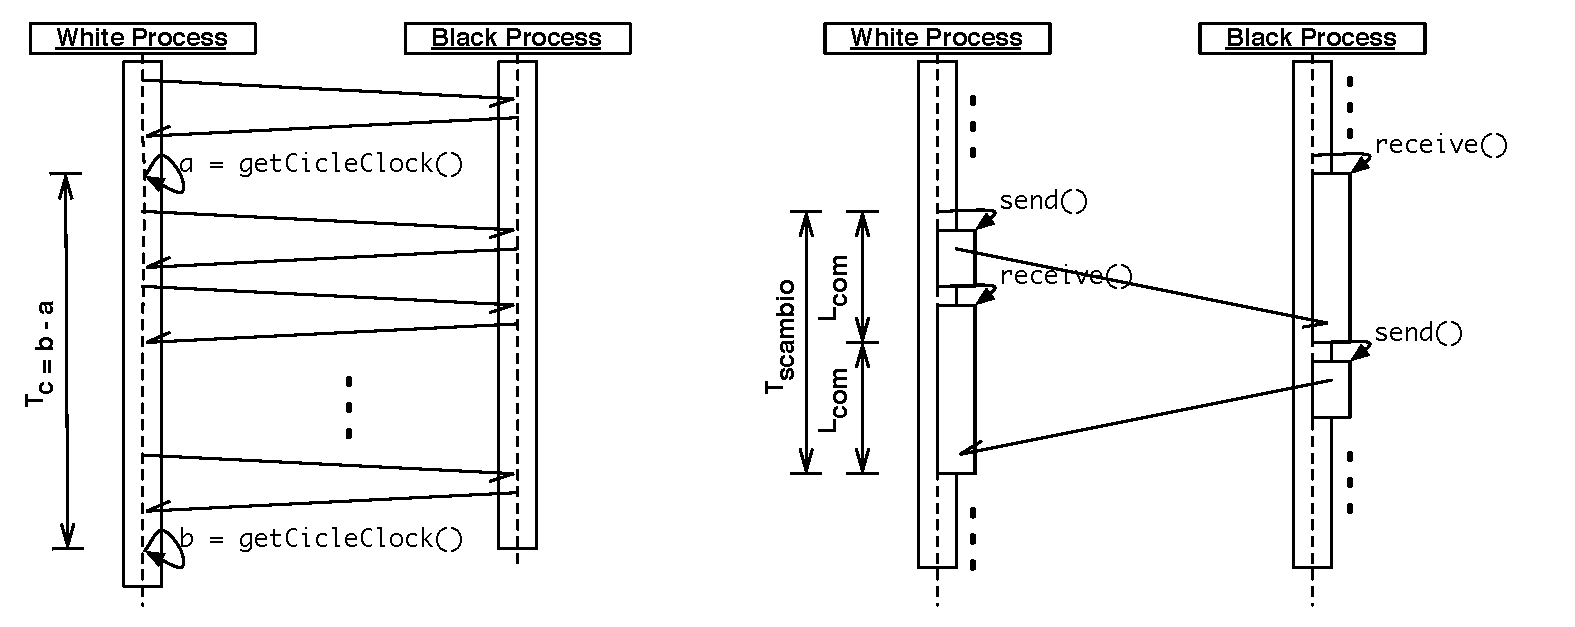
\includegraphics[scale=.5]{schema_metering.pdf}
  \caption[Comportamento temporale dell'applicazione ``ping-pong'']{Rappresentazione della sequenza di azioni svolte dai due processi dell'applicazione di misurazione. A sinistra viene mostrato il comportamento complessivo, a destra il dettaglio di uno scambio di messaggi.}
  \label{fig:schema_metering}
\end{figure}

Il programma di misurazione effettua $m$ scambi di messaggi. L'esecuzione e la corrispondente misurazione del tempo di completamento degli scambi \`e eseguita per diverse configurazioni di allocazione dei processi nei PE, a distanze diverse nella mesh. I valori di distanza, o \emph{numero di hops}, considerati sono: il minimo (1), il massimo (14) e quello medio ($\sqrt{64} = 8$). Per ogni configurazione vengono eseguite $n$ misure, ad ogni iterazione viene calcolato il valore medio della latenza di comunicazione per gli $m$ scambi effettuati. Per ogni distanza viene presentata la media, il valore massimo e la devianza standard degli $n$ valori medi della latenza di comunicazione. 

Nella misurazione della comunicazione asimmetrica si prendono in considerazione solo le due principali implementazioni del supporto, ovvero quella che fa uso della UDN e quella che utilizza al meglio la memoria condivisa \footnote{Per determinare questa informazione si usano i risultati della misura delle implementazioni simmetriche, si veda la discussione nella sezione~\ref{sct:meter_risultati}}. Inoltre, per la stessa forma di comunicazione e per quanto riguarda l'implementazione su memoria condivisa, viene fornita un'altra misura, chiamata \verb+ch_asymin_sm_all+. Viene utilizzato un canale asimmetrico con il massimo numero di processi mittenti allocabili nella macchina; come in precedenza, la misura \`e effettuata con lo scambio di messaggi tra due soli processi. La misura \`e interessante in quanto la politica di ricezione del destinatario prevede la scansione del flag \verb+Rdy+ di tutti i processi mittenti. \`E pertanto auspicabile un aumento della latenza di comunicazione con l'aumento del numero dei mittenti, anche se solo uno di questi comunica con il destinatario. Si osserva che questo secondo modo di misurare la comunicazione asimmetrica non fornisce risultati significati per l'implementazione UDN, e per questo motivo non \`e mostrato nei risultati. Con l'uso di UDN, infatti, la politica di ricezione non deterministica da pi\`u mittenti \`e implementata nativamente dal firmware della macchina e non \`e soggetta a overhead (\`e la lettura da una coda FIFO di registri).


\subsubsection{Risultati}
\label{sct:meter_risultati}
\begin{figure}[p]
  \centering
  \begin{subfigure}[b]{.5\textheight}
    %% $ cd meter_data
    %% $ ./compact 2_4_*.dat
    %% $ ./printAll  2 4
    %% $ ./plot.sh 2 4
    %% $ cd ..
    %% $ cp meter_data/2_4_{sym,asymin}_all.{tex,pdf} ./
    \resizebox{\columnwidth}{!}{% GNUPLOT: LaTeX picture with Postscript
\begingroup
  \makeatletter
  \providecommand\color[2][]{%
    \GenericError{(gnuplot) \space\space\space\@spaces}{%
      Package color not loaded in conjunction with
      terminal option `colourtext'%
    }{See the gnuplot documentation for explanation.%
    }{Either use 'blacktext' in gnuplot or load the package
      color.sty in LaTeX.}%
    \renewcommand\color[2][]{}%
  }%
  \providecommand\includegraphics[2][]{%
    \GenericError{(gnuplot) \space\space\space\@spaces}{%
      Package graphicx or graphics not loaded%
    }{See the gnuplot documentation for explanation.%
    }{The gnuplot epslatex terminal needs graphicx.sty or graphics.sty.}%
    \renewcommand\includegraphics[2][]{}%
  }%
  \providecommand\rotatebox[2]{#2}%
  \@ifundefined{ifGPcolor}{%
    \newif\ifGPcolor
    \GPcolortrue
  }{}%
  \@ifundefined{ifGPblacktext}{%
    \newif\ifGPblacktext
    \GPblacktexttrue
  }{}%
  % define a \g@addto@macro without @ in the name:
  \let\gplgaddtomacro\g@addto@macro
  % define empty templates for all commands taking text:
  \gdef\gplbacktext{}%
  \gdef\gplfronttext{}%
  \makeatother
  \ifGPblacktext
    % no textcolor at all
    \def\colorrgb#1{}%
    \def\colorgray#1{}%
  \else
    % gray or color?
    \ifGPcolor
      \def\colorrgb#1{\color[rgb]{#1}}%
      \def\colorgray#1{\color[gray]{#1}}%
      \expandafter\def\csname LTw\endcsname{\color{white}}%
      \expandafter\def\csname LTb\endcsname{\color{black}}%
      \expandafter\def\csname LTa\endcsname{\color{black}}%
      \expandafter\def\csname LT0\endcsname{\color[rgb]{1,0,0}}%
      \expandafter\def\csname LT1\endcsname{\color[rgb]{0,1,0}}%
      \expandafter\def\csname LT2\endcsname{\color[rgb]{0,0,1}}%
      \expandafter\def\csname LT3\endcsname{\color[rgb]{1,0,1}}%
      \expandafter\def\csname LT4\endcsname{\color[rgb]{0,1,1}}%
      \expandafter\def\csname LT5\endcsname{\color[rgb]{1,1,0}}%
      \expandafter\def\csname LT6\endcsname{\color[rgb]{0,0,0}}%
      \expandafter\def\csname LT7\endcsname{\color[rgb]{1,0.3,0}}%
      \expandafter\def\csname LT8\endcsname{\color[rgb]{0.5,0.5,0.5}}%
    \else
      % gray
      \def\colorrgb#1{\color{black}}%
      \def\colorgray#1{\color[gray]{#1}}%
      \expandafter\def\csname LTw\endcsname{\color{white}}%
      \expandafter\def\csname LTb\endcsname{\color{black}}%
      \expandafter\def\csname LTa\endcsname{\color{black}}%
      \expandafter\def\csname LT0\endcsname{\color{black}}%
      \expandafter\def\csname LT1\endcsname{\color{black}}%
      \expandafter\def\csname LT2\endcsname{\color{black}}%
      \expandafter\def\csname LT3\endcsname{\color{black}}%
      \expandafter\def\csname LT4\endcsname{\color{black}}%
      \expandafter\def\csname LT5\endcsname{\color{black}}%
      \expandafter\def\csname LT6\endcsname{\color{black}}%
      \expandafter\def\csname LT7\endcsname{\color{black}}%
      \expandafter\def\csname LT8\endcsname{\color{black}}%
    \fi
  \fi
  \setlength{\unitlength}{0.0500bp}%
  \begin{picture}(7200.00,5040.00)%
    \gplgaddtomacro\gplbacktext{%
      \csname LTb\endcsname%
      \put(946,704){\makebox(0,0)[r]{\strut{} 0}}%
      \put(946,1128){\makebox(0,0)[r]{\strut{} 50}}%
      \put(946,1553){\makebox(0,0)[r]{\strut{} 100}}%
      \put(946,1977){\makebox(0,0)[r]{\strut{} 150}}%
      \put(946,2402){\makebox(0,0)[r]{\strut{} 200}}%
      \put(946,2826){\makebox(0,0)[r]{\strut{} 250}}%
      \put(946,3251){\makebox(0,0)[r]{\strut{} 300}}%
      \put(946,3675){\makebox(0,0)[r]{\strut{} 350}}%
      \put(2223,484){\makebox(0,0){\strut{}1}}%
      \put(3369,484){\makebox(0,0){\strut{}8}}%
      \put(4514,484){\makebox(0,0){\strut{}14}}%
      \put(5791,704){\makebox(0,0)[l]{\strut{} 0}}%
      \put(5791,1071){\makebox(0,0)[l]{\strut{} 0.05}}%
      \put(5791,1438){\makebox(0,0)[l]{\strut{} 0.1}}%
      \put(5791,1805){\makebox(0,0)[l]{\strut{} 0.15}}%
      \put(5791,2172){\makebox(0,0)[l]{\strut{} 0.2}}%
      \put(5791,2539){\makebox(0,0)[l]{\strut{} 0.25}}%
      \put(5791,2906){\makebox(0,0)[l]{\strut{} 0.3}}%
      \put(5791,3273){\makebox(0,0)[l]{\strut{} 0.35}}%
      \put(5791,3640){\makebox(0,0)[l]{\strut{} 0.4}}%
      \put(176,2189){\rotatebox{-270}{\makebox(0,0){\strut{}$\mathrm{L}_{\mathrm{com}} \; (\,\tau\,)$}}}%
      \put(6692,2189){\rotatebox{-270}{\makebox(0,0){\strut{}$\mathrm{L}_{\mathrm{com}} \; (\,\mu\mathrm{sec}\,)$}}}%
      \put(3368,154){\makebox(0,0){\strut{}number of hops}}%
    }%
    \gplgaddtomacro\gplfronttext{%
      \csname LTb\endcsname%
      \put(4804,4867){\makebox(0,0)[r]{\strut{}\texttt{ch\_sym\_udn}}}%
      \csname LTb\endcsname%
      \put(4804,4647){\makebox(0,0)[r]{\strut{}\texttt{ch\_sym\_sm\_rdyack\_no}}}%
      \csname LTb\endcsname%
      \put(4804,4427){\makebox(0,0)[r]{\strut{}\texttt{ch\_sym\_sm\_rdyack}}}%
      \csname LTb\endcsname%
      \put(4804,4207){\makebox(0,0)[r]{\strut{}\texttt{ch\_sym\_sm\_nullack}}}%
    }%
    \gplbacktext
    \put(0,0){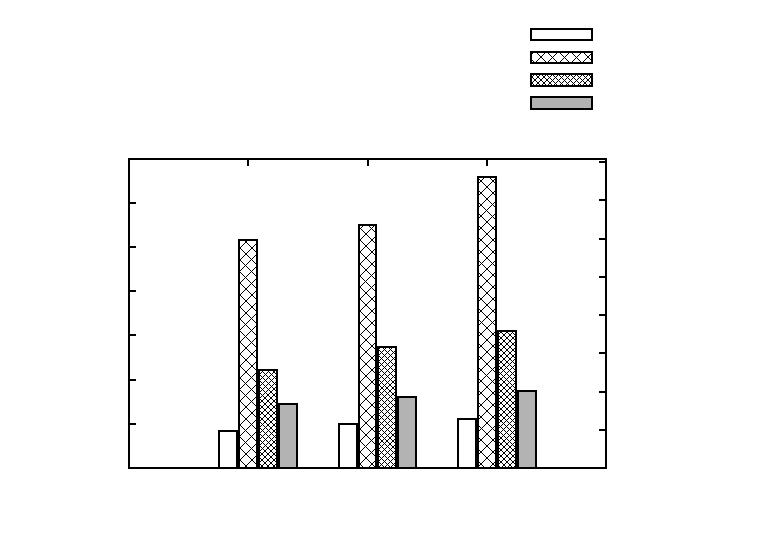
\includegraphics{2_5_sym_all_bw}}%
    \gplfronttext
  \end{picture}%
\endgroup
}
    \caption{Latenza di comunicazione misurata delle implementazioni del canale simmetrico}
    \label{fig:meter_ch_sym_2_4}
  \end{subfigure}
  \\
  \vspace{1cm}
  \begin{subfigure}[b]{.5\textheight}
    \resizebox{\columnwidth}{!}{% GNUPLOT: LaTeX picture with Postscript
\begingroup
  \makeatletter
  \providecommand\color[2][]{%
    \GenericError{(gnuplot) \space\space\space\@spaces}{%
      Package color not loaded in conjunction with
      terminal option `colourtext'%
    }{See the gnuplot documentation for explanation.%
    }{Either use 'blacktext' in gnuplot or load the package
      color.sty in LaTeX.}%
    \renewcommand\color[2][]{}%
  }%
  \providecommand\includegraphics[2][]{%
    \GenericError{(gnuplot) \space\space\space\@spaces}{%
      Package graphicx or graphics not loaded%
    }{See the gnuplot documentation for explanation.%
    }{The gnuplot epslatex terminal needs graphicx.sty or graphics.sty.}%
    \renewcommand\includegraphics[2][]{}%
  }%
  \providecommand\rotatebox[2]{#2}%
  \@ifundefined{ifGPcolor}{%
    \newif\ifGPcolor
    \GPcolortrue
  }{}%
  \@ifundefined{ifGPblacktext}{%
    \newif\ifGPblacktext
    \GPblacktexttrue
  }{}%
  % define a \g@addto@macro without @ in the name:
  \let\gplgaddtomacro\g@addto@macro
  % define empty templates for all commands taking text:
  \gdef\gplbacktext{}%
  \gdef\gplfronttext{}%
  \makeatother
  \ifGPblacktext
    % no textcolor at all
    \def\colorrgb#1{}%
    \def\colorgray#1{}%
  \else
    % gray or color?
    \ifGPcolor
      \def\colorrgb#1{\color[rgb]{#1}}%
      \def\colorgray#1{\color[gray]{#1}}%
      \expandafter\def\csname LTw\endcsname{\color{white}}%
      \expandafter\def\csname LTb\endcsname{\color{black}}%
      \expandafter\def\csname LTa\endcsname{\color{black}}%
      \expandafter\def\csname LT0\endcsname{\color[rgb]{1,0,0}}%
      \expandafter\def\csname LT1\endcsname{\color[rgb]{0,1,0}}%
      \expandafter\def\csname LT2\endcsname{\color[rgb]{0,0,1}}%
      \expandafter\def\csname LT3\endcsname{\color[rgb]{1,0,1}}%
      \expandafter\def\csname LT4\endcsname{\color[rgb]{0,1,1}}%
      \expandafter\def\csname LT5\endcsname{\color[rgb]{1,1,0}}%
      \expandafter\def\csname LT6\endcsname{\color[rgb]{0,0,0}}%
      \expandafter\def\csname LT7\endcsname{\color[rgb]{1,0.3,0}}%
      \expandafter\def\csname LT8\endcsname{\color[rgb]{0.5,0.5,0.5}}%
    \else
      % gray
      \def\colorrgb#1{\color{black}}%
      \def\colorgray#1{\color[gray]{#1}}%
      \expandafter\def\csname LTw\endcsname{\color{white}}%
      \expandafter\def\csname LTb\endcsname{\color{black}}%
      \expandafter\def\csname LTa\endcsname{\color{black}}%
      \expandafter\def\csname LT0\endcsname{\color{black}}%
      \expandafter\def\csname LT1\endcsname{\color{black}}%
      \expandafter\def\csname LT2\endcsname{\color{black}}%
      \expandafter\def\csname LT3\endcsname{\color{black}}%
      \expandafter\def\csname LT4\endcsname{\color{black}}%
      \expandafter\def\csname LT5\endcsname{\color{black}}%
      \expandafter\def\csname LT6\endcsname{\color{black}}%
      \expandafter\def\csname LT7\endcsname{\color{black}}%
      \expandafter\def\csname LT8\endcsname{\color{black}}%
    \fi
  \fi
  \setlength{\unitlength}{0.0500bp}%
  \begin{picture}(7200.00,5040.00)%
    \gplgaddtomacro\gplbacktext{%
      \csname LTb\endcsname%
      \put(946,704){\makebox(0,0)[r]{\strut{} 0}}%
      \put(946,1059){\makebox(0,0)[r]{\strut{} 50}}%
      \put(946,1413){\makebox(0,0)[r]{\strut{} 100}}%
      \put(946,1768){\makebox(0,0)[r]{\strut{} 150}}%
      \put(946,2122){\makebox(0,0)[r]{\strut{} 200}}%
      \put(946,2477){\makebox(0,0)[r]{\strut{} 250}}%
      \put(946,2831){\makebox(0,0)[r]{\strut{} 300}}%
      \put(946,3186){\makebox(0,0)[r]{\strut{} 350}}%
      \put(946,3540){\makebox(0,0)[r]{\strut{} 400}}%
      \put(946,3895){\makebox(0,0)[r]{\strut{} 450}}%
      \put(2256,484){\makebox(0,0){\strut{}1}}%
      \put(3435,484){\makebox(0,0){\strut{}8}}%
      \put(4613,484){\makebox(0,0){\strut{}14}}%
      \put(5923,704){\makebox(0,0)[l]{\strut{} 0}}%
      \put(5923,1317){\makebox(0,0)[l]{\strut{} 0.1}}%
      \put(5923,1930){\makebox(0,0)[l]{\strut{} 0.2}}%
      \put(5923,2543){\makebox(0,0)[l]{\strut{} 0.3}}%
      \put(5923,3156){\makebox(0,0)[l]{\strut{} 0.4}}%
      \put(5923,3769){\makebox(0,0)[l]{\strut{} 0.5}}%
      \put(176,2299){\rotatebox{-270}{\makebox(0,0){\strut{}$\mathrm{L}_{\mathrm{com}} \; (\,\tau\,)$}}}%
      \put(6692,2299){\rotatebox{-270}{\makebox(0,0){\strut{}$\mathrm{L}_{\mathrm{com}} \; (\,\mu\mathrm{sec}\,)$}}}%
      \put(3434,154){\makebox(0,0){\strut{}number of hops}}%
    }%
    \gplgaddtomacro\gplfronttext{%
      \csname LTb\endcsname%
      \put(4936,4867){\makebox(0,0)[r]{\strut{}\texttt{ch\_asymin\_udn}}}%
      \csname LTb\endcsname%
      \put(4936,4647){\makebox(0,0)[r]{\strut{}\texttt{ch\_asymin\_sm\_all}}}%
      \csname LTb\endcsname%
      \put(4936,4427){\makebox(0,0)[r]{\strut{}\texttt{ch\_asymin\_sm}}}%
    }%
    \gplbacktext
    \put(0,0){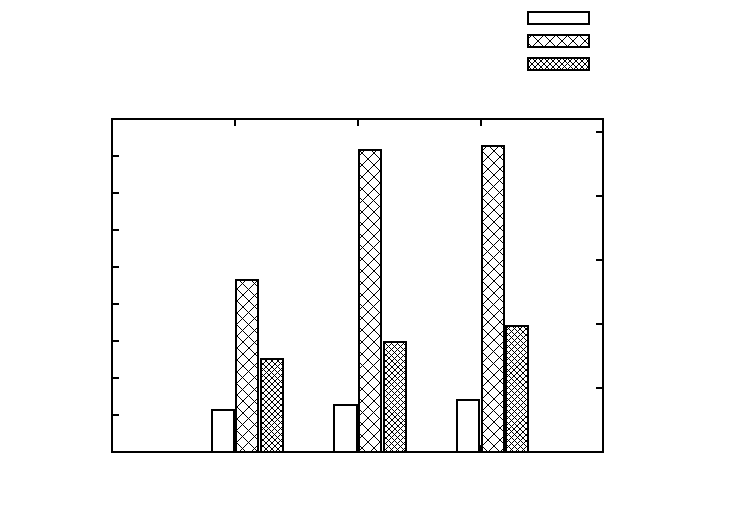
\includegraphics{2_5_asymin_all_bw}}%
    \gplfronttext
  \end{picture}%
\endgroup
}
    \caption{Latenza di comunicazione misurata delle implementazioni del canale asimmetrico in ingresso}
    \label{fig:meter_ch_asymin_2_4}
  \end{subfigure}
  \caption[Latenza di comunicazione dei canali]{Rappresentazione grafica dei risultati delle misurazioni della latenza di comunicazione dei canali. Il programma di misurazione \`e stato eseguito con un numero $m = 10^5$ di scambi e un numero $n = 10$ di iterazioni.}
  \label{fig:meter_type2_nscamb4}
\end{figure}

\begin{table}[!b]
  \centering
  \begin{subtable}[b]{\textwidth}
    \centering
    \begin{tabular}{|l|r|r|r|r|r|}
      \hline
      \multirow{3}{*}{\emph{Implementazione}} &
      \multirow{3}{4ex}{\emph{\# Hops}} &
      \multicolumn{4}{|c|}{$\inLcom$} \\
      \cline{3-6}
      & & \multicolumn{2}{|c|}{\emph{Avg}} &
      \multirow{2}{*}{\emph{Std Dev}} &
      \multirow{2}{*}{\emph{Max} $(\,\tau\,)$} \\
      \cline{3-4}
      & & $\tau$ & $\mu\mathrm{sec}$ & & \\
      \hline
      %% \multirow{3}{18ex}{\texttt{ch\_sym\_udn}} 
      %% & 1 & 42.066550 & 0.048655 & 0.097822 & 42.262000 \\
      %% & 8 & 49.561120 & 0.057323 & 0.104196 & 49.769500 \\
      %% & 14 & 55.722760 & 0.064450 & 0.107943 & 55.792050 \\
      %% \hline
      %% \multirow{3}{18ex}{\texttt{ch\_sym\_sm\_rdyack\_no}} 
      %% & 1 & 257.800490 & 0.298178 & 0.008955 & 257.815900 \\
      %% & 8 & 275.320380 & 0.318442 & 0.006685 & 275.327650 \\
      %% & 14 & 329.332180 & 0.380914 & 0.018220 & 329.363400 \\
      %% \hline
      %% \multirow{3}{18ex}{\texttt{ch\_sym\_rdyack\_sm}}
      %% & 1 & 111.482450 & 0.128943 & 0.187050 & 111.653200 \\
      %% & 8 & 137.378440 & 0.158895 & 0.016294 & 137.395550 \\
      %% & 14 & 155.377520 & 0.179713 & 0.013281 & 155.393950 \\
      %% \hline
      %% \multirow{3}{18ex}{\texttt{ch\_sym\_sm\_nullack}}
      %% & 1 & 72.359500 & 0.083692 & 0.219423 & 72.549500 \\ 
      %% & 8 & 80.700840 & 0.093340 & 0.124463 & 80.827350 \\ 
      %% & 14 & 86.759230 & 0.100347 & 0.118203 & 86.826250 \\
      \multirow{3}{*}{\texttt{ch\_sym\_udn}} 
      & 1 & 42.067 & 0.04866 & 0.09782 & 42.262 \\
      & 8 & 49.561 & 0.05732 & 0.10419 & 49.770 \\
      & 14 & 55.723 & 0.06445 & 0.10794 & 55.792 \\
      \hline
      \multirow{3}{*}{\texttt{ch\_sym\_sm\_rdyack\_no}} 
      & 1 & 257.800 & 0.29818 & 0.00896 & 257.816 \\
      & 8 & 275.320 & 0.31844 & 0.00669 & 275.328 \\
      & 14 & 329.332 & 0.38091 & 0.01822 & 329.363 \\
      \hline
      \multirow{3}{*}{\texttt{ch\_sym\_rdyack\_sm}}
      & 1 & 111.482 & 0.12894 & 0.18701 & 111.653 \\
      & 8 & 137.378 & 0.15890 & 0.01633 & 137.396 \\
      & 14 & 155.378 & 0.17971 & 0.01328 & 155.394 \\
      \hline
      \multirow{3}{*}{\texttt{ch\_sym\_sm\_nullack}}
      & 1 & 72.360 & 0.08369 & 0.21942 & 72.550 \\ 
      & 8 & 80.701 & 0.09334 & 0.12446 & 80.827 \\ 
      & 14 & 86.759 & 0.10034 & 0.11820 & 86.826 \\
      \hline
    \end{tabular}
    \caption[Latenza dei canali di comunicazione simmetrici]{Misurazione della latenza di comunicazione simmetrica delle diverse implementazioni.}
  \end{subtable}

  %%%%%%%%%%%%%%%%%%%%%%%%%%%%%%%%%%%%%%%%%%%%%%%%%%%%%%%%%%%%%%%%%%%%%%%%%%%%%%%%
  \vspace{4ex}
  %%%%%%%%%%%%%%%%%%%%%%%%%%%%%%%%%%%%%%%%%%%%%%%%%%%%%%%%%%%%%%%%%%%%%%%%%%%%%%%%

  \begin{subtable}[b]{\textwidth}
    \centering
    \begin{tabular}{|l|r|r|r|r|r|}
      \hline
      \multirow{3}{*}{\emph{Implementazione}} &
      \multirow{3}{4ex}{\emph{\# Hops}} &
      \multicolumn{4}{|c|}{$\inLcom$} \\
      \cline{3-6}
      & & \multicolumn{2}{|c|}{\emph{Avg}} &
      \multirow{2}{*}{\emph{Std Dev}} &
      \multirow{2}{*}{\emph{Max} $(\,\tau\,)$} \\
      \cline{3-4}
      & & $\tau$ & $\mu\mathrm{sec}$ & & \\
      \hline
      %% \multirow{3}{*}{\texttt{ch\_asymin\_udn}}
      %% & 1 & 56.025529 & 0.064800 & 0.000941 & 56.026905 \\
      %% & 8 & 63.525349 & 0.073475 & 0.000979 & 63.526575 \\
      %% & 14 & 69.527121 & 0.080416 & 0.001011 & 69.528720 \\
      %% \hline
      %% \multirow{3}{*}{\texttt{ch\_asymin\_sm\_all}}
      %% & 1 & 230.570268 & 0.266683 & 0.028743 & 230.643940 \\
      %% & 8 & 408.779285 & 0.472804 & 0.047859 & 408.846645 \\
      %% & 14 & 414.374837 & 0.479276 & 0.025326 & 414.417200 \\
      %% \hline
      %% \multirow{3}{*}{\texttt{ch\_asymin\_sm}}
      %% & 1 & 125.039207 & 0.144623 & 0.001632 & 125.041220 \\
      %% & 8 & 149.041103 & 0.172384 & 0.001936 & 149.045050 \\
      %% & 14 & 170.037299 & 0.196669 & 0.002036 & 170.040285 \\
      \multirow{3}{*}{\texttt{ch\_asymin\_udn}}
      & 1 & 56.0255 & 0.06480 & 0.00094 & 56.027 \\
      & 8 & 63.525 & 0.07348 & 0.00098 & 63.527 \\
      & 14 & 69.527 & 0.08042 & 0.00101 & 69.529 \\
      \hline
      \multirow{3}{*}{\texttt{ch\_asymin\_sm\_all}}
      & 1 & 230.570 & 0.26668 & 0.02874 & 230.644 \\
      & 8 & 408.779 & 0.47280 & 0.04786 & 408.847 \\
      & 14 & 414.375 & 0.47928 & 0.02533 & 414.417 \\
      \hline
      \multirow{3}{*}{\texttt{ch\_asymin\_sm}}
      & 1 & 125.039 & 0.14462 & 0.00163 & 125.041 \\
      & 8 & 149.041 & 0.17238 & 0.00194 & 149.045 \\
      & 14 & 170.037 & 0.19667 & 0.00204 & 170.040 \\
      \hline
    \end{tabular}
    \caption{Misurazione della latenza di comunicazione asimmetrica in ingresso delle diverse implementazioni.}
  \end{subtable}

  \caption[Latenza dei canali di comunicazione asimmetrici]{Misure della latenza di comunicazione rilevate iterando 10 volte il programma ``ping-pong'' con $m = 10^5$ scambi }
  \label{tab:meter}
\end{table}

I risultati proposti in tabella~\ref{tab:meter} e graficamente in figura~\ref{fig:meter_type2_nscamb4}, sono relativi a 10 iterazioni del programma di misurazione con $m = 10^5$ scambi di messaggi tra i due processi.

I risultati ottenuti verificano i ragionamenti descritti nelle Sezioni \ref{sct:specifica_sm}, \ref{sct:specifica_udn} che hanno guidato la realizzazione delle diverse implementazioni. La prima considerazione riguarda il confronto tra l'uso della UDN e della memoria condivisa: in entrambe le forme di comunicazione l'implementazione di UDN ha latenza inferiore a quella dell'implementazione con memoria condivisa pi\`u veloce. Raffiniamo questa osservazione valutando quale sia la migliore implementazione su memoria condivisa e quindi confrontiamola con l'implementazione UDN. La migliore implementazione su SM non \`e necessariamente quella pi\`u veloce: sebbene il protocollo Null-Ack fornisca la minor latenza, la sua implementazione fa uso di un valore particolare dei messaggi e pertanto \`e meno generica delle altre implementazioni. Ad esempio se si richiedesse una implementazione di canali di tipo generico, l'applicazione di questo protocollo potrebbe essere problematica. L'implementazione Null-Ack \`e utile per conoscere quale \`e la degradazione introdotta dalla barriera di memoria, necessaria nel protocollo Rdy-Ack, e quindi quale \`e il vero overhead della nostra implementazione lock-free dei canali. 

Passiamo a valutare la differenza tra le due implementazioni su SM che usano il protocollo Rdy-Ack e che differiscono per la gestione della gerarchia cache. Una gestione esplicita dell'allocazione in cache, che massimizzi la localit\`a dei dati, dimezza la latenza di comunicazione rispetto alla gestione predefinita dell'allocazione. Questo \`e un risultato generale, l'impostazione del PE consumatore come Home per il dato acceduto in computazioni \emph{consumatore~-~produttore} risulta determinante per ottimizzare le prestazioni; considerazioni simili sono state valutate in contesti differenti \cite{buono2013parallel}. Consideriamo quindi la \verb+ch_sym_sm_rdyack+ come implementazione candidata su memoria condivisa, che usa il protocollo Rdy-Ack. Osserviamo che il rapporto tra la latenza di questa soluzione e quella con il protocollo Null-Ack (sempre su SM) \`e di 1.68. Dato che le due implementazioni eseguono istruzioni simili, con la solo differenza della barriera di memoria, \`e ragionevole valutare la causa di questo aumento della latenza come l'esecuzione della memory fence.\\
Si osserva inoltre che l'implementazione Rdy-Ack \`e leggermente pi\`u sensibile alla variazione di distanza dei due processi, rispetto alla Null-Ack; quest'ultima ha un aumento della latenza pari a tanti cicli di clock quanto \`e l'aumento della distanza. Si nota che in questo aspetto la Null-Ack si comporta come la UDN. 
%%La seconda osservazione sulle implementazioni SM riguarda la gestione esplicita della gerarchia cache al fine di massimizzare la localit\`a dei dati: questa possibilit\`a risulta essere fondamentale per le prestazioni su memoria condivisa. L'uso della gestione predefinita \`e due volte pi\`u lento della versione con il descrittore di canale partizionato e homed nelle caches consumatori. \\
%%Si considera \verb+ch_sym_sm_rdyack+ l'implementazione migliore su SM. 

Si considera infine il rapporto tra la soluzione su SM e quella su UDN. Il vantaggio di uso dell'implementazione UDN rispetto a quella SM \`e significativo: mediamente la latenza UDN \`e inferiore pi\`u della met\`a (1/2.737) di quella SM. 

Il confronto dei canali asimmetrici con un singolo mittente ha risultato simile al confronto precedente. In questo caso il rapporto medio tra la latenze UDN e quella SM, 1/2.341, \`e leggermente maggiore. \`E significativo anche il confronto tra questi canali e i corrispondenti simmetrici, in quanto, nel programma di misurazione, i canali asimmetrici sono utilizzati per realizzare forme di comunicazione simmetrica. In entrambi i casi si ha un aumento della latenza di circa 10 cicli di clock. Ci\`o pu\`o essere spiegato dalle specifiche implementazioni parallele: con l'uso della UDN il mittente invia due parole, anzich\`e una del caso simmetrico; con l'uso della SM abbiamo l'uso di altre variabili, ad esempio per garantire la fairness, rispetto al caso simmetrico. \\
Si osserva infine che esiste una differenza sostanziale tra l'uso del canale asimmetrico su SM con un singolo mittente rispetto a quello con tutti i mittenti, ma uno solo attivo. La latenza nel secondo caso \`e mediamente il doppio di quella con un singolo mittente, ne segue un divario ancora pi\`u ampio con la latenza del canale su UDN.\\



%% media dei rapporti tra rdyack e nullack 1.678
%% media dei rapporti tra rdyack_no e rdy ack 2.145
%% media dei rapporti tra udn e rdyack 2.737
%% media dei rapporti tra asym_udn e asym_sm 2.341
%% media dei rapporti tra asym_udn e asym_sm_all 5.503





%% \begin{figure}[!h]
%%   \centering
%%   \resizebox{\columnwidth}{!}{% GNUPLOT: LaTeX picture with Postscript
\begingroup
  \makeatletter
  \providecommand\color[2][]{%
    \GenericError{(gnuplot) \space\space\space\@spaces}{%
      Package color not loaded in conjunction with
      terminal option `colourtext'%
    }{See the gnuplot documentation for explanation.%
    }{Either use 'blacktext' in gnuplot or load the package
      color.sty in LaTeX.}%
    \renewcommand\color[2][]{}%
  }%
  \providecommand\includegraphics[2][]{%
    \GenericError{(gnuplot) \space\space\space\@spaces}{%
      Package graphicx or graphics not loaded%
    }{See the gnuplot documentation for explanation.%
    }{The gnuplot epslatex terminal needs graphicx.sty or graphics.sty.}%
    \renewcommand\includegraphics[2][]{}%
  }%
  \providecommand\rotatebox[2]{#2}%
  \@ifundefined{ifGPcolor}{%
    \newif\ifGPcolor
    \GPcolortrue
  }{}%
  \@ifundefined{ifGPblacktext}{%
    \newif\ifGPblacktext
    \GPblacktexttrue
  }{}%
  % define a \g@addto@macro without @ in the name:
  \let\gplgaddtomacro\g@addto@macro
  % define empty templates for all commands taking text:
  \gdef\gplbacktext{}%
  \gdef\gplfronttext{}%
  \makeatother
  \ifGPblacktext
    % no textcolor at all
    \def\colorrgb#1{}%
    \def\colorgray#1{}%
  \else
    % gray or color?
    \ifGPcolor
      \def\colorrgb#1{\color[rgb]{#1}}%
      \def\colorgray#1{\color[gray]{#1}}%
      \expandafter\def\csname LTw\endcsname{\color{white}}%
      \expandafter\def\csname LTb\endcsname{\color{black}}%
      \expandafter\def\csname LTa\endcsname{\color{black}}%
      \expandafter\def\csname LT0\endcsname{\color[rgb]{1,0,0}}%
      \expandafter\def\csname LT1\endcsname{\color[rgb]{0,1,0}}%
      \expandafter\def\csname LT2\endcsname{\color[rgb]{0,0,1}}%
      \expandafter\def\csname LT3\endcsname{\color[rgb]{1,0,1}}%
      \expandafter\def\csname LT4\endcsname{\color[rgb]{0,1,1}}%
      \expandafter\def\csname LT5\endcsname{\color[rgb]{1,1,0}}%
      \expandafter\def\csname LT6\endcsname{\color[rgb]{0,0,0}}%
      \expandafter\def\csname LT7\endcsname{\color[rgb]{1,0.3,0}}%
      \expandafter\def\csname LT8\endcsname{\color[rgb]{0.5,0.5,0.5}}%
    \else
      % gray
      \def\colorrgb#1{\color{black}}%
      \def\colorgray#1{\color[gray]{#1}}%
      \expandafter\def\csname LTw\endcsname{\color{white}}%
      \expandafter\def\csname LTb\endcsname{\color{black}}%
      \expandafter\def\csname LTa\endcsname{\color{black}}%
      \expandafter\def\csname LT0\endcsname{\color{black}}%
      \expandafter\def\csname LT1\endcsname{\color{black}}%
      \expandafter\def\csname LT2\endcsname{\color{black}}%
      \expandafter\def\csname LT3\endcsname{\color{black}}%
      \expandafter\def\csname LT4\endcsname{\color{black}}%
      \expandafter\def\csname LT5\endcsname{\color{black}}%
      \expandafter\def\csname LT6\endcsname{\color{black}}%
      \expandafter\def\csname LT7\endcsname{\color{black}}%
      \expandafter\def\csname LT8\endcsname{\color{black}}%
    \fi
  \fi
  \setlength{\unitlength}{0.0500bp}%
  \begin{picture}(7200.00,5040.00)%
    \gplgaddtomacro\gplbacktext{%
      \csname LTb\endcsname%
      \put(946,704){\makebox(0,0)[r]{\strut{} 0}}%
      \put(946,1128){\makebox(0,0)[r]{\strut{} 50}}%
      \put(946,1553){\makebox(0,0)[r]{\strut{} 100}}%
      \put(946,1977){\makebox(0,0)[r]{\strut{} 150}}%
      \put(946,2402){\makebox(0,0)[r]{\strut{} 200}}%
      \put(946,2826){\makebox(0,0)[r]{\strut{} 250}}%
      \put(946,3251){\makebox(0,0)[r]{\strut{} 300}}%
      \put(946,3675){\makebox(0,0)[r]{\strut{} 350}}%
      \put(2223,484){\makebox(0,0){\strut{}1}}%
      \put(3369,484){\makebox(0,0){\strut{}8}}%
      \put(4514,484){\makebox(0,0){\strut{}14}}%
      \put(5791,704){\makebox(0,0)[l]{\strut{} 0}}%
      \put(5791,1071){\makebox(0,0)[l]{\strut{} 0.05}}%
      \put(5791,1438){\makebox(0,0)[l]{\strut{} 0.1}}%
      \put(5791,1805){\makebox(0,0)[l]{\strut{} 0.15}}%
      \put(5791,2172){\makebox(0,0)[l]{\strut{} 0.2}}%
      \put(5791,2539){\makebox(0,0)[l]{\strut{} 0.25}}%
      \put(5791,2906){\makebox(0,0)[l]{\strut{} 0.3}}%
      \put(5791,3273){\makebox(0,0)[l]{\strut{} 0.35}}%
      \put(5791,3640){\makebox(0,0)[l]{\strut{} 0.4}}%
      \put(176,2189){\rotatebox{-270}{\makebox(0,0){\strut{}$\mathrm{L}_{\mathrm{com}} \; (\,\tau\,)$}}}%
      \put(6692,2189){\rotatebox{-270}{\makebox(0,0){\strut{}$\mathrm{L}_{\mathrm{com}} \; (\,\mu\mathrm{sec}\,)$}}}%
      \put(3368,154){\makebox(0,0){\strut{}number of hops}}%
    }%
    \gplgaddtomacro\gplfronttext{%
      \csname LTb\endcsname%
      \put(4261,4867){\makebox(0,0)[r]{\strut{}\texttt{ch\_sym\_udn}}}%
      \csname LTb\endcsname%
      \put(4261,4647){\makebox(0,0)[r]{\strut{}\texttt{ch\_sym\_sm\_rdyack\_no}}}%
      \csname LTb\endcsname%
      \put(4261,4427){\makebox(0,0)[r]{\strut{}\texttt{ch\_sym\_sm\_rdyack}}}%
      \csname LTb\endcsname%
      \put(4261,4207){\makebox(0,0)[r]{\strut{}\texttt{ch\_sym\_sm\_nullack}}}%
    }%
    \gplbacktext
    \put(0,0){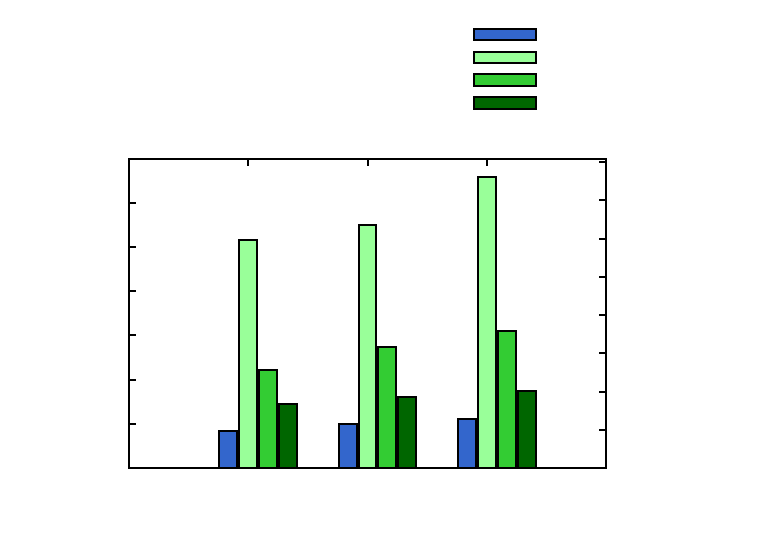
\includegraphics{2_5_sym_all}}%
    \gplfronttext
  \end{picture}%
\endgroup
}
%%   \caption{}
%%   \label{fig:meter_ch_sym_2_5}
%% \end{figure}

%% \begin{figure}[!hb]
%%   \centering
%%   \resizebox{\columnwidth}{!}{% GNUPLOT: LaTeX picture with Postscript
\begingroup
  \makeatletter
  \providecommand\color[2][]{%
    \GenericError{(gnuplot) \space\space\space\@spaces}{%
      Package color not loaded in conjunction with
      terminal option `colourtext'%
    }{See the gnuplot documentation for explanation.%
    }{Either use 'blacktext' in gnuplot or load the package
      color.sty in LaTeX.}%
    \renewcommand\color[2][]{}%
  }%
  \providecommand\includegraphics[2][]{%
    \GenericError{(gnuplot) \space\space\space\@spaces}{%
      Package graphicx or graphics not loaded%
    }{See the gnuplot documentation for explanation.%
    }{The gnuplot epslatex terminal needs graphicx.sty or graphics.sty.}%
    \renewcommand\includegraphics[2][]{}%
  }%
  \providecommand\rotatebox[2]{#2}%
  \@ifundefined{ifGPcolor}{%
    \newif\ifGPcolor
    \GPcolortrue
  }{}%
  \@ifundefined{ifGPblacktext}{%
    \newif\ifGPblacktext
    \GPblacktexttrue
  }{}%
  % define a \g@addto@macro without @ in the name:
  \let\gplgaddtomacro\g@addto@macro
  % define empty templates for all commands taking text:
  \gdef\gplbacktext{}%
  \gdef\gplfronttext{}%
  \makeatother
  \ifGPblacktext
    % no textcolor at all
    \def\colorrgb#1{}%
    \def\colorgray#1{}%
  \else
    % gray or color?
    \ifGPcolor
      \def\colorrgb#1{\color[rgb]{#1}}%
      \def\colorgray#1{\color[gray]{#1}}%
      \expandafter\def\csname LTw\endcsname{\color{white}}%
      \expandafter\def\csname LTb\endcsname{\color{black}}%
      \expandafter\def\csname LTa\endcsname{\color{black}}%
      \expandafter\def\csname LT0\endcsname{\color[rgb]{1,0,0}}%
      \expandafter\def\csname LT1\endcsname{\color[rgb]{0,1,0}}%
      \expandafter\def\csname LT2\endcsname{\color[rgb]{0,0,1}}%
      \expandafter\def\csname LT3\endcsname{\color[rgb]{1,0,1}}%
      \expandafter\def\csname LT4\endcsname{\color[rgb]{0,1,1}}%
      \expandafter\def\csname LT5\endcsname{\color[rgb]{1,1,0}}%
      \expandafter\def\csname LT6\endcsname{\color[rgb]{0,0,0}}%
      \expandafter\def\csname LT7\endcsname{\color[rgb]{1,0.3,0}}%
      \expandafter\def\csname LT8\endcsname{\color[rgb]{0.5,0.5,0.5}}%
    \else
      % gray
      \def\colorrgb#1{\color{black}}%
      \def\colorgray#1{\color[gray]{#1}}%
      \expandafter\def\csname LTw\endcsname{\color{white}}%
      \expandafter\def\csname LTb\endcsname{\color{black}}%
      \expandafter\def\csname LTa\endcsname{\color{black}}%
      \expandafter\def\csname LT0\endcsname{\color{black}}%
      \expandafter\def\csname LT1\endcsname{\color{black}}%
      \expandafter\def\csname LT2\endcsname{\color{black}}%
      \expandafter\def\csname LT3\endcsname{\color{black}}%
      \expandafter\def\csname LT4\endcsname{\color{black}}%
      \expandafter\def\csname LT5\endcsname{\color{black}}%
      \expandafter\def\csname LT6\endcsname{\color{black}}%
      \expandafter\def\csname LT7\endcsname{\color{black}}%
      \expandafter\def\csname LT8\endcsname{\color{black}}%
    \fi
  \fi
  \setlength{\unitlength}{0.0500bp}%
  \begin{picture}(7200.00,5040.00)%
    \gplgaddtomacro\gplbacktext{%
      \csname LTb\endcsname%
      \put(946,704){\makebox(0,0)[r]{\strut{} 0}}%
      \put(946,1059){\makebox(0,0)[r]{\strut{} 50}}%
      \put(946,1413){\makebox(0,0)[r]{\strut{} 100}}%
      \put(946,1768){\makebox(0,0)[r]{\strut{} 150}}%
      \put(946,2122){\makebox(0,0)[r]{\strut{} 200}}%
      \put(946,2477){\makebox(0,0)[r]{\strut{} 250}}%
      \put(946,2831){\makebox(0,0)[r]{\strut{} 300}}%
      \put(946,3186){\makebox(0,0)[r]{\strut{} 350}}%
      \put(946,3540){\makebox(0,0)[r]{\strut{} 400}}%
      \put(946,3895){\makebox(0,0)[r]{\strut{} 450}}%
      \put(2256,484){\makebox(0,0){\strut{}1}}%
      \put(3435,484){\makebox(0,0){\strut{}8}}%
      \put(4613,484){\makebox(0,0){\strut{}14}}%
      \put(5923,704){\makebox(0,0)[l]{\strut{} 0}}%
      \put(5923,1317){\makebox(0,0)[l]{\strut{} 0.1}}%
      \put(5923,1930){\makebox(0,0)[l]{\strut{} 0.2}}%
      \put(5923,2543){\makebox(0,0)[l]{\strut{} 0.3}}%
      \put(5923,3156){\makebox(0,0)[l]{\strut{} 0.4}}%
      \put(5923,3769){\makebox(0,0)[l]{\strut{} 0.5}}%
      \put(176,2299){\rotatebox{-270}{\makebox(0,0){\strut{}$\mathrm{L}_{\mathrm{com}} \; (\,\tau\,)$}}}%
      \put(6692,2299){\rotatebox{-270}{\makebox(0,0){\strut{}$\mathrm{L}_{\mathrm{com}} \; (\,\mu\mathrm{sec}\,)$}}}%
      \put(3434,154){\makebox(0,0){\strut{}number of hops}}%
    }%
    \gplgaddtomacro\gplfronttext{%
      \csname LTb\endcsname%
      \put(4129,4867){\makebox(0,0)[r]{\strut{}\texttt{ch\_asymin\_udn}}}%
      \csname LTb\endcsname%
      \put(4129,4647){\makebox(0,0)[r]{\strut{}\texttt{ch\_asymin\_sm\_all}}}%
      \csname LTb\endcsname%
      \put(4129,4427){\makebox(0,0)[r]{\strut{}\texttt{ch\_asymin\_sm}}}%
    }%
    \gplbacktext
    \put(0,0){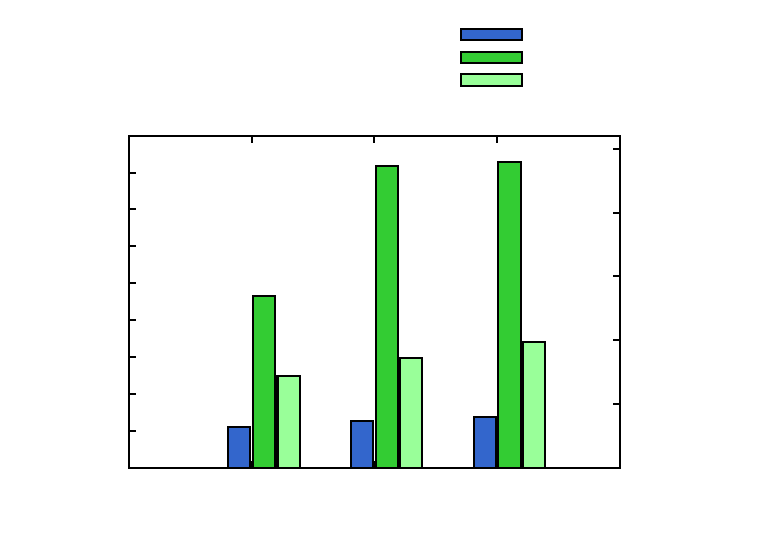
\includegraphics{2_5_asymin_all}}%
    \gplfronttext
  \end{picture}%
\endgroup
}
%%   \caption{}
%%   \label{fig:meter_ch_asymin_2_5}
%% \end{figure}


%%%%%%%%%%%%%%%%%%%%%%%%%%%%%%%%%%%%%%%%%%%%%%%%%%%%%%%%%%%%%%%%%%%%%%%%%%%%%%%%


  
\FloatBarrier


%% \begin{table}[!h]
%%   \centering
%%   \begin{tabular}{|l|l|l|l|l|}
%%     \hline
%%     \multirow{2}{22ex}{\emph{Implemenatation}} & \multirow{2}{*}{\emph{\#Hops}} & \multicolumn{3}{|c|}{$\inLcom \; (\tau)$} \\
%%     \cline{3-5}
%%     & & \emph{Avg} & \emph{Std Dev} & \emph{Max} \\
%%     \hline
%%     \multirow{3}{18ex}{\texttt{ch\_asymin\_udn}} & \\
%%     & \\
%%     & \\
%%     \hline
%%     \multirow{3}{18ex}{\texttt{ch\_asymin\_sm\_no}} & \\
%%     & \\
%%     & \\
%%     \hline
%%     \multirow{3}{18ex}{\texttt{ch\_asymin\_sm}} & \\
%%     & \\
%%     & \\
%%     \hline
%%   \end{tabular}
%%   \caption{Risultati numerici, in cicli di clock, della misurazione della latenza di comunicazione asimmetrica in ingresso delle diverse implementazioni.}
%% \end{table}



%% \begin{table}[!h]
%%   \centering
%%   \begin{subtable}[b]{\textwidth}
%%     \begin{tabular}{|l|l|l|l|l|}
%%       \hline
%%       \multirow{2}{22ex}{\emph{Implemenatation}} & \multirow{2}{*}{\emph{\#Hops}} & \multicolumn{3}{|c|}{$\inLcom \; (\tau)$} \\
%%       \cline{3-5}
%%       & & \emph{Avg} & \emph{Std Dev} & \emph{Max} \\
%%       \hline
%%       \multirow{3}{18ex}{\texttt{ch\_sym\_udn}} & 1 & 42.066550 & 0.097822 & 42.262000 \\
%%       & 8 & 49.561120 & 0.104196 & 49.769500 \\
%%       & 14 & 55.722760 & 0.107943 & 55.792050 \\
%%       \hline
%%       \multirow{3}{18ex}{\texttt{ch\_sym\_sm\_no}} & 1 & 257.800490 & 0.008955 & 257.815900 \\
%%       & 8 & 275.320380 & 0.006685 & 275.327650 \\
%%       & 14 & 329.332180 & 0.018220 & 329.363400 \\
%%       \hline
%%       \multirow{3}{18ex}{\texttt{ch\_sym\_sm}} & 1 & 111.482450 & 0.187050 & 111.653200 \\
%%       & 8 & 137.378440 & 0.016294 & 137.395550 \\
%%       & 14 & 155.377520 & 0.013281 & 155.393950 \\
%%       \hline
%%       \multirow{3}{18ex}{\texttt{ch\_sym\_sm\_nullack}} & 1 & 72.359500 & 0.219423 & 72.549500 \\ 
%%       & 8 & 80.700840 & 0.124463 & 80.827350 \\ 
%%       & 14 & 86.759230 & 0.118203 & 86.826250 \\
%%       \hline
%%     \end{tabular}
%%     \caption{Misurazione della latenza di comunicazione simmetrica delle diverse implementazioni.}
%%   \end{subtable}

%%   %%%%%%%%%%%%%%%%%%%%%%%%%%%%%%%%%%%%%%%%%%%%%%%%%%%%%%%%%%%%%%%%%%%%%%%%%%%%%%%%
%%   \vspace{4ex}
%%   %%%%%%%%%%%%%%%%%%%%%%%%%%%%%%%%%%%%%%%%%%%%%%%%%%%%%%%%%%%%%%%%%%%%%%%%%%%%%%%%

%%   \begin{subtable}[b]{\textwidth}
%%     \centering
%%     \begin{tabular}{|l|l|l|l|l|}
%%       \hline
%%       \multirow{2}{22ex}{\emph{Implemenatation}} & \multirow{2}{*}{\emph{\#Hops}} & \multicolumn{3}{|c|}{$\inLcom \; (\tau)$} \\
%%       \cline{3-5}
%%       & & \emph{Avg} & \emph{Std Dev} & \emph{Max} \\
%%       \hline
%%       \multirow{3}{18ex}{\texttt{ch\_asymin\_udn}} & 1 & 56.025529 & 0.000941 & 56.026905 \\
%%       & 8 & 63.525349 & 0.000979 & 63.526575 \\
%%       & 14 & 69.527121 & 0.001011 & 69.528720 \\
%%       \hline
%%       \multirow{3}{18ex}{\texttt{ch\_asymin\_sm\_all}} & 1 & 230.570268 & 0.028743 & 230.643940 \\
%%       & 8 & 408.779285 & 0.047859 & 408.846645 \\
%%       & 14 & 414.374837 & 0.025326 & 414.417200 \\
%%       \hline
%%       \multirow{3}{18ex}{\texttt{ch\_asymin\_sm}} & 1 & 125.039207 & 0.001632 & 125.041220 \\
%%       & 8 & 149.041103 & 0.001936 & 149.045050 \\
%%       & 14 & 170.037299 & 0.002036 & 170.040285 \\
%%       \hline
%%     \end{tabular}
%%     \caption{Misurazione della latenza di comunicazione asimmetrica in ingresso delle diverse implementazioni.}
%%   \end{subtable}

%%   \caption{Misure della latenza di comunicazione rilevate iterando 10 volte il programma ``ping-pong'' con $m = 10^5$ scambi }

%% \end{table}




\null
\vfill
\newpage

\subsection{Benchmark moltiplicazione matrice-vettore}
In questa sezione viene proposto un secondo esperimento volto a verificare il comportamento delle implementazioni del supporto su SM e su UDN in una applicazione realistica, con un numero di processi parametrico e potenzialmente alto (fino al massimo numero di PE disponibili, visto l'uso del mapping esclusivo). In particolare \`e stata scelta una applicazione sintetizzata per mezzo di paradigmi di parallelismo che faccia uso sia di comunicazioni simmetriche e di almeno una comunicazione asimmetrica in ingresso. Per mostrare le differenze prestazionali delle due implementazioni la computazione scelta ha calcoli di grana fine e prevede l'elaborazione di dati su stream. Per lo stesso programma sono state eseguite due versioni che utilizzano rispettivamente: solo il supporto alle comunicazioni su SM, e solo il supporto alle comunicazioni su UDN. La principale metrica per il confronto di queste due esecuzioni \`e il tempo di completamento della computazione al variare della dimensione dei dati e del numero di processi usati.

\subsubsection{Descrizione del problema}
Il benchmark proposto si basa su un calcolo numerico di algebra lineare molto frequente nella risoluzione di problemi reali, non solo in ambito scientifico: il prodotto matrice per vettore. Sia $\mathbf{A} = (a_{ij})_{i=1,\ldots,\mathrm{M}, j=1,\ldots,\mathrm{M}} \in \mathbb{Z}^{\mathrm{MxM}}$ una matrice di interi di dimensione MxM, e sia $\mathbf{b} = (b_1,\ldots,b_\mathrm{M}) \in \mathbb{Z}^{\mathrm{M}}$ un vettore di M interi, il risultato dell'operazione prodotto matrice per vettore \`e un vettore $\mathbf{c} = (c_1,\ldots,c_\mathrm{M}) = \mathbf{A} \cdot \mathbf{b} \in \mathbb{Z^{M}}$ la cui componente $i$-esima \`e il prodotto scalare tra la riga $i$-esima di $\mathbf{A}$ e il vettore $\mathbf{b}$.
\[ \forall \; i \in \{1,\ldots,\mathrm{M}\} \; : \; c_i = \mathbf{a}_i \cdot \mathbf{b} = \sum_{j=1}^{\mathrm{M}} a_{ij} \cdot b_j  \]
Dove $\mathbf{a}_i = (a_{i1},\ldots,a_{i\mathrm{M}})$ \`e la riga $i$-esima della matrice $\mathbf{A}$. Da questa definizione segue direttamente l'algoritmo sequenziale del calcolo, che \`e descritto dal codice~\ref{lst:benchmark_seq_alg}.\\
\begin{lstlisting}[float = b, morekeywords = {to}, caption = {Algoritmo sequenziale del calcolo matrice per vettore}, label={lst:benchmark_seq_alg}]
int A[M][M], b[M], c[M];
for i:=0 to M-1 do 
  c[i] := 0;
  for j:=0 to M-1 do
    c[i] := A[i][j]*b[j] + c[i];
\end{lstlisting}

\begin{figure}[!tb]
  \centering
  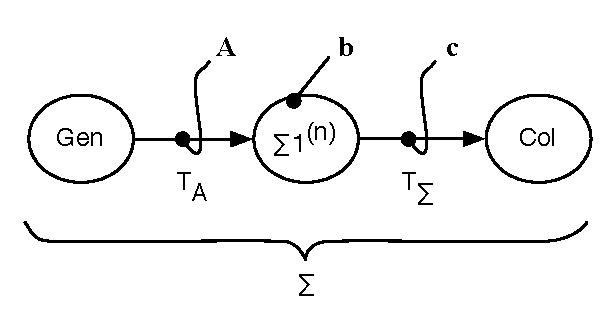
\includegraphics[scale=.5]{grafo_sigma_compatto.pdf}
  \caption[Computazione sequenziale del benchmark]{Rappresentazione compatta del grafo della computazione. L'elemento $\Sigma1$ \`e un modulo sequenziale o un sottosistema parallelo che esegue la moltiplicazione per $\mathbf{b}$ su ogni elemento della matrice. }
  \label{fig:sigma_compatto}
\end{figure}
La computazione considerata riguarda un sistema $\Sigma$ modellato come un grafo aciclico contenente un modulo di elaborazione collegato a due stream, uno di ingresso e l'altro di uscita. Lo stream di ingresso \`e composto da $m$ matrici di interi di dimensione fissata MxM e con un tempo medio di interarrivo \Ta, lo stream di uscita invece trasporta i risultati del calcolo eseguito dal modulo. Su ogni elemento dello stream il modulo calcola la moltiplicazione matrice per vettore utilizzando l'elemento stesso come primo operando e un vettore $\mathbf{b}$, costante per tutta la durata dell'applicazione, come secondo operando. Il vettore risultato di ogni operazione viene scritto nello stream di uscita. 
Ci poniamo nel caso in cui il tempo di calcolo di una moltiplicazione matrice per vettore, \Tcalc, sia superiore al tempo di interarrivo \Ta. Dato che il tempo di servizio della computazione $\Sigma$ \`e  superiore a quello ideale (il tempo di interarrivo dello stream \footnote{Per una trattazione formale della valutazione delle prestazioni di computazioni su stream in grafi aciclici si consulti \cite{hpc_part1}}), si richiede una trasformazione del modulo sequenziale in un sottosistema parallelo funzionalmente equivalente che permetta di eliminare o ridurre il collo di bottiglia nel sistema, determinato dal modulo stesso, e mantenga massima l'efficienza del sottosistema. 
Si indica con \subsystem\ il sottosistema parallelo di calcolo, con grado di parallelismo $n$. 
Dal punto di vista teorico e indipendentemente dalla soluzione parallela scelta, si ha che il tempo di servizio \emph{ideale} del sottosistema parallelo \`e il rapporto tra tempo di calcolo del programma sequenziale e il grado di parallelismo (equazione \ref{eq:TsubsysId}). Il tempo di servizio effettivo del sottosistema \`e invece il massimo valore tra il tempo medio di interarrivo dello stream e il tempo di servizio ideale del sottosistema (equazione \ref{eq:Tsubsys}). Si definisce \emph{efficienza} del sottosistema il rapporto tra i tempi di servizio ideale ed effettivo (equazione \ref{eq:subsysEff}). Ne segue che il sottosistema ha efficienza massima 
%% quando il collo di bottiglia non \`e eliminato dal sottositema, 
se e solo se nella computazione rimane il collo di bottiglia, 
ovvero il grado di parallelismo \emph{non} \`e sufficientemente alto affinch\`e il tempo di servizio ideale sia minore o uguale del tempo di interarrivo. 
Altrimenti, se il collo di bottiglia \`e stato eliminato, l'efficienza non \`e massima e il suo valore corrisponde al \emph{fattore di utilizzazione} del sottosistema, ovvero il rapporto tra il tempo di servizio ideale del sottosistema e il tempo di interarrivo. Da tale caratterizzazione ne segue il valore ottimo del grado di parallelismo, ovvero quel valore di $n$ che consente di eliminare il collo di bottiglia e mantenere massima l'efficienza del sottosistema (equazione \ref{eq:nopt}).
\begin{flalign}
  \label{eq:TsubsysId}
  \inTsubsystemId &= \inTs = \frac{\inTcalc}{n} \\
  \label{eq:Tsubsys}
  \inTsubsystem &= \max(\{\inTa, \; \inTs \}) \\
  \label{eq:subsysEff}
  \inEffic &= \frac{\inTsubsystemId}{\inTsubsystem} = \left\{ \begin{array}{ll} \frac{\inTs}{\inTa}, & \inTs < \inTa \\ 1, & \inTs \ge \inTa \end{array} \right. \in (0,\ldots,1] \\
  \label{eq:nopt}
  n_{\mathrm{opt}} \; &= \; \min(\{ n \in \mathbb{N} \;\, | \;\, \inTs \le \inTa \}) \; = \; \left\lceil \frac{\inTcalc}{\inTa} \right\rceil
\end{flalign}
\\

Altre definizioni utili per caratterizzare le prestazioni dell'applicazione sono le seguenti:
\begin{description}
\item [Tempo di completamento dello stream] \`e definita come il tempo medio impiegato per completare l'esecuzione del calcolo su tutti gli elementi dello stream. Se la lunghezza dello stream $m$ \`e molto superiore al grado di parallelismo $n$ \`e possibile approssimarlo come m volte il tempo medio di servizio del sistema
\begin{equation}
\label{eq:Tc}
m >> n \quad \Rightarrow \quad \inTc = m \cdot \inTsystem
\end{equation}
\item [Scalabilit\`a] esprime il risparmio relativo del tempo medio di servizio che pu\`o essere ottenuto usando l'implementazione parallela con $n$ processi rispetto all'implementazione sequenziale. Pu\`o essere espressa anche in termini del tempo di completamento.
\begin{flalign}
\label{eq:s}
s^{(n)} &= \frac{\inTcalc}{\inTsystem} \\
\label{eq:sId}
s_{\mathrm{id}}^{\phantom{id}(n)} &= \frac{\inTcalc}{\inTsystemId} = \frac{\inTcalc}{\frac{\inTcalc}{n}} = n
\end{flalign}  
%% The speedup of a parallel implementation expresses the relative saving of execution time that can be obtained by using a parallel execution on p processors compared to the best sequential implementation.

\end{description}

\subsubsection{Sul problema scelto}
\begin{figure}[!t]
  \begin{subfigure}[b]{.5\textwidth}
    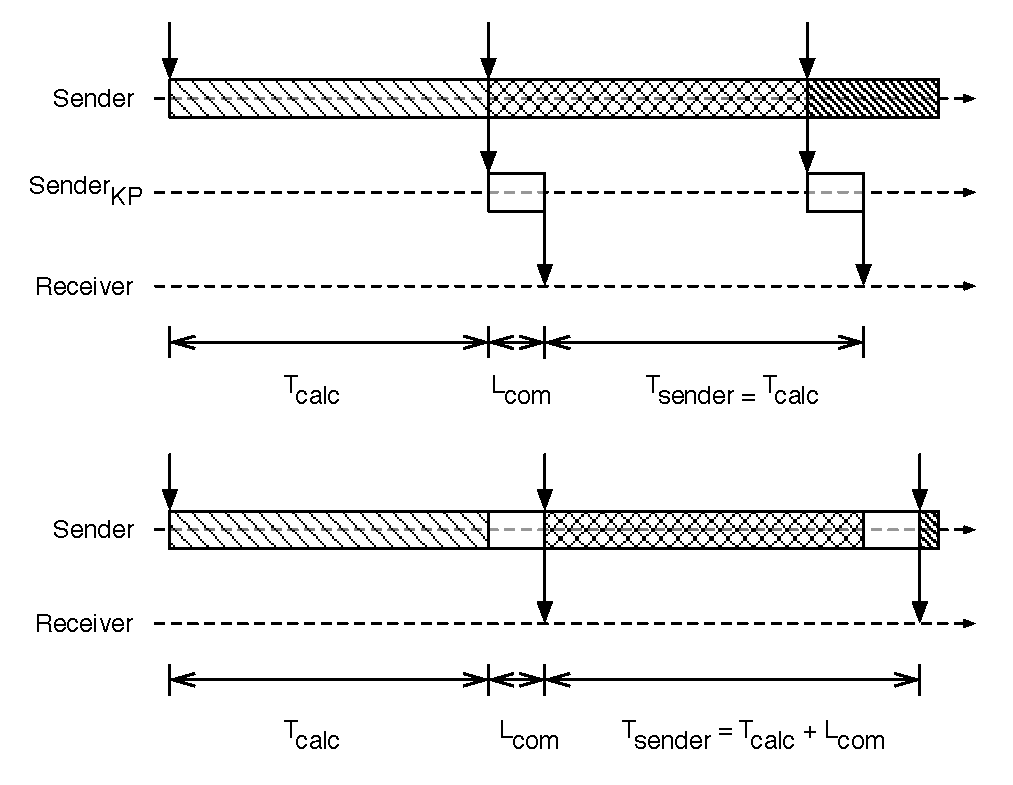
\includegraphics[scale=.38]{servicetime_eg_coarse-grain.pdf}
    \caption{Calcolo di grana grossa}
    \label{fig:eg_coarse_grain}
  \end{subfigure}
  ~
  \begin{subfigure}[b]{.5\textwidth}
    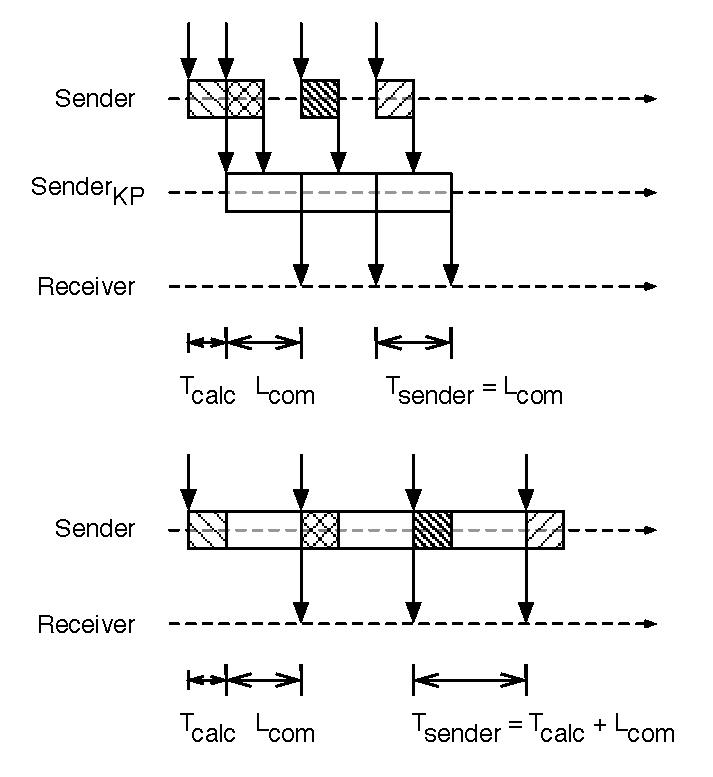
\includegraphics[scale=.38]{servicetime_eg_fine-grain.pdf}
    \caption{Calcolo di grana fine}
    \label{fig:eg_fine_grain}
  \end{subfigure}
  \caption[Esempio di due computazioni su stream con diversa grana]{Rappresentazione grafica di due computazioni con diversa ``grana'' di calcolo, in presenza e in assenza di un processore di comunicazione}
  \label{fig:eg_grain}
\end{figure}
\`E importante soffermarci e motivare il tipo di applicazione scelta: il supporto alle comunicazioni fornito \`e specifico per un dominio applicativo caratterizzato da grana di calcolo fine, se non finissima. Solo in computazioni di questo tipo siamo interessati a ridurre la latenza di comunicazione, e si osservano quindi delle differenze nelle prestazioni globali dell'applicazione. A scopo esemplificativo si considera una parte di una applicazione su stream riguardante due moduli collegati in pipeline: si assume che il tempo di calcolo del primo modulo sia opportunamente dimensionato come il tempo di interarrivo dello stream. Le figure~\ref{fig:eg_coarse_grain},~\ref{fig:eg_fine_grain} mostrano due situazioni con diversa grana di calcolo del primo modulo. Se il tempo di calcolo \`e di diversi ordini di grandezza superiore alla latenza di comunicazione, l'ottimizzazione di qualche centinaio di cicli di clock della comunicazione non consegue alcun vantaggio sul tempo di servizio effettivo del modulo; la comunicazione avr\`a sempre impatto nullo o trascurabile nel tempo di servizio effettivo del modulo. Se \`e possibile la sovrapposizione del calcolo infatti la latenza di comunicazione \`e completamente mascherata dal tempo di calcolo, altrimenti, la latenza di comunicazione si va a sommare al tempo di calcolo, risultando trascurabile. L'ottimizzazione delle comunicazioni \`e invece apprezzabile quando la latenza di queste \`e dello stesso ordine di grandezza del tempo di calcolo. 

Computazioni di grana fine sono molto frequenti nel dominio delle applicazioni su stream di elementi, si pensi a forme di deep packet inspection nel campo della computer networking, nelle quali vengono esaminati specifiche parti di pacchetti, che passano da un punto di ispezione di una rete di computer, alla ricerca di non conformit\`a, o per collezionare statistiche sulle informazioni trasmesse. Computazioni su dato singolo, in special modo quelle che seguono il paradigma Data Parallel sono caratterizzate da grana fine delle computazioni, in seguito al partizionamento del dato. Anche in queste applicazioni \`e utile disporre di un supporto efficiente alle comunicazioni, sia per le forme di comunicazione collettiva, che per le comunicazioni tra moduli in caso di dipendenze sui dati (forme Stencil).

Il Benchmark \`e stato scelto nell'ottica di apprezzare le differenze tra le due realizzazioni del supporto e di verificare il loro comportamento in una applicazione reale. Le due implementazioni del supporto non differiscono solo dal conseguimento di una diversa latenza di comunicazione, come mostrato nell'esperimento precedente. La versione UDN permette un disaccoppiamento tra la comunicazione dei processi e l'accesso ai dati in memoria. La comunicazione tra due processi \`e realizzata interamente con l'uso della UDN e senza l'impiego della memoria condivisa. Ci\`o ha come effetto un numero di richieste alla memoria condivisa minore rispetto all'implementazione dei canali con la memoria. Ci aspettiamo che questo fatto abbia ripercussioni positive sulle prestazioni globali dell'applicazione, non solo per quanto riguarda le comunicazioni, ma in pi\`u in generale, relativamente al tempo di risposta delle richieste alla memoria.
  

\subsubsection{Il metodo di parallelizzazione scelto}
La parallelizzazione del modulo sequenziale \`e stata scelta tra un insieme ristretto (per il tipo di computazione) di paradigmi la cui semantica e modello dei costi sono noti \cite{hpc_part1}, tra cui:
\begin{description}
\item [Farm] \`e caratterizzata dalla replicazione della funzione di calcolo sequenziale in $n$ identiche unit\`a di elaborazione (sottoinsieme delle unit\`a worker). \`E applicabile solo a computazioni su stream, viene usata una unit\`a emettitore per la distribuzione di un elemento dello stream ad un worker, e una unit\`a collettore, collegata ad ogni worker, per ricevere i risultati;
\item [Data Parallel] sono forme di parallelismo che richiedono una discreta conoscenza del calcolo sequenziale ma che per questo motivo risultano flessibili alla specifica computazione. Si basano sul partizionamento dei dati e sulla replicazione della funzione di calcolo nelle unit\`a worker, possono essere applicate sia a singoli dati che a stream di dati; in quest'ultimo caso il partizionamento \`e applicato ad ogni elemento dello stream. I gradi di libert\`a forniti riguardano la strategia di partizionamento dei dati, l'eventuale replicazione di dati, l'organizzazione delle unit\`a worker (indipendenti o interagenti) e il collezionamento dei risultati parziali. Vengono usate forme di comunicazione collettiva per distribuire le partizioni del dato (\emph{scatter}), per collezionare i risultati parziali (\emph{gather}) e/o per costruire il risultato (ad esempio l'operazione di \emph{reduce}). A seconda dell'organizzazione dei workers si distinguono due famiglie di forme Data Parallel: \emph{Map} se ogni worker esegue un calcolo completamente indipendente da quello degli altri worker, \emph{Stencil-based} se esiste un'interazione tra i workers durante l'esecuzione del calcolo.
\end{description}
Si \`e deciso di adottare un paradigma di tipo Data Parallel cos\`i da poter applicare il supporto alle comunicazioni per la realizzazione delle comunicazioni collettive coinvolte, in modo da confrontare le prestazioni dei due tipi di supporto forniti anche relativamente all'implementazione di tali comunicazioni. In particolare, il collezionamento dei risultati sar\`a realizzato per mezzo di un canale asimmetrico in ingresso che ha come mittenti l'insieme dei processi worker dell'implementazione Data Parallel, e come destinatario un processo collettore. Come spiegato in seguito si rende necessaria una distribuzione di ciascun elemento dello stream ai processi worker, piuttosto che una distribuzione delle partizioni di ogni elemento. L'implementazione di questa operazione fa uso dei canali simmetrici ed \`e caratterizzata da una struttura ad albero mappata sull'insieme dei worker. \\

Analizzando le dipendenze sui dati del programma sequenziale (codice~\ref{lst:benchmark_seq_alg}) si osserva che una qualsiasi istruzione di una certa iterazione del ciclo esterno \`e indipendente da tutte le istruzioni di un'altra qualsiasi iterazione dello stesso ciclo. Al contrario ogni istruzione di una iterazione del ciclo interno dipende (\emph{Read-After-Write}) dall'istruzione precedente della stessa iterazione.
\begin{lstlisting}[caption={Rappresentazione delle istruzioni di due cicli esterni contigui.}]
...
{ c[i]:=0; c[i]:=A[i][0]*b[0]+c[i]; c[i]:=A[i][1]*b[1]+c[i]; ... c[i]:=A[i][M-1]*b[M-1]+c[i]; }
{ c[i+1]:=0; c[i+1]:=A[i+1][0]*b[0]+c[i+1]; ... c[i+1]:=A[i+1][M-1]*b[M-1]+c[i+1]; }
...
\end{lstlisting}
Ne segue che pu\`o essere esplicitato del parallelismo sul ciclo esterno, eseguendo iterazioni diverse del ciclo esterno in processi diversi, ottenendo in tal modo un grado massimo di parallelismo $n = \textrm{M}$ e una complessit\`a di esecuzione $O(n)$ contro $O(n^2)$ del calcolo sequenziale. Da ci\`o deriva direttamente il partizionamento delle matrici, che \`e per righe. In tale situazione si ha la ``grana'' minima sia per quanto riguarda le partizioni dei dati, che per il tempo di calcolo.
In generale, un'implementazione effettiva fa uso di un grado di parallelismo $n$ minore di M, dipendentemente dal valore medio del tempo di interarrivo dello stream. In tale situazione le matrici sono sempre partizionate per riga, con grana $g = \lceil M / n \rceil$ righe, il calcolo dei processi worker consiste di $g$ prodotti scalari tra ogni riga della partizione associata al worker e il vettore $\mathbf{b}$. 

Si adotta la replicazione del vettore $\mathbf{b}$ nei processi worker, ci\`o \`e possibile in quanto tale oggetto viene acceduto in sola lettura. Di conseguenza l'implementazione Data Parallel descritta \`e di tipo \emph{Map}. \\

Rispetto a quanto detto finora il sottosistema Map \`e caratterizzato da una comunicazione di \emph{multicast} piuttosto che dalla scatter; infatti si utilizza il supporto alle comunicazioni descritto nella sezione~\ref{sct:specifica_meccanismi} per realizzare gli archi del grafo,
%% \marginpar{RENDERE MEGLIO}
 conseguentemente abbiamo il sottografo Map operante su uno stream di riferimenti. Lo stream di ingresso trasporter\`a i riferimenti alle matrici, la distribuzione di un elemento dello stream ai moduli della Map \`e quindi l'invio dello stesso riferimento agli $n$ moduli; sar\`a poi dovere di ogni worker eseguire il calcolo sulla propria partizione dell'oggetto riferito dal puntatore ricevuto in ingresso. \\

L'implementazione pi\`u semplice della distribuzione multicast fa uso di un singolo processo distributore che in modo sequenziale esegue l'invio del dato ad ogni processo worker. Questa soluzione \`e critica per comunicazioni di grana fine, in quanto pu\`o diventare rapidamente un collo di bottiglia all'aumentare del grado di parallelismo. Considerato l'ambito di applicazioni in si pone il supporto \`e lecito aspettarsi stream caratterizzati da elevata banda, quindi la necessit\`a di disporre di comunicazioni collettive (tra cui la multicast) efficienti, che non siano collo di bottiglia per l'applicazione. Implementazioni della multicast adeguate a questo contesto hanno tempo di servizio costante, ad esempio implementano il processo distributore come un sottosistema parallelo strutturato ad albero. In questo caso, grazie all'effetto-pipeline, il tempo di servizio \`e pari alla latenza di comunicazione di un canale simmetrico per l'ariet\`a dell'albero. Ci\`o richiedere tuttavia nodi aggiuntivi a quelli del sottosistema parallelo. Una soluzione alternativa che mantenga lo stesso tempo di servizio senza moduli addizionali consiste nell'implementare l'albero in modo distribuito direttamente nell'insieme dei moduli worker.
\begin{figure}[!t]
  \centering
  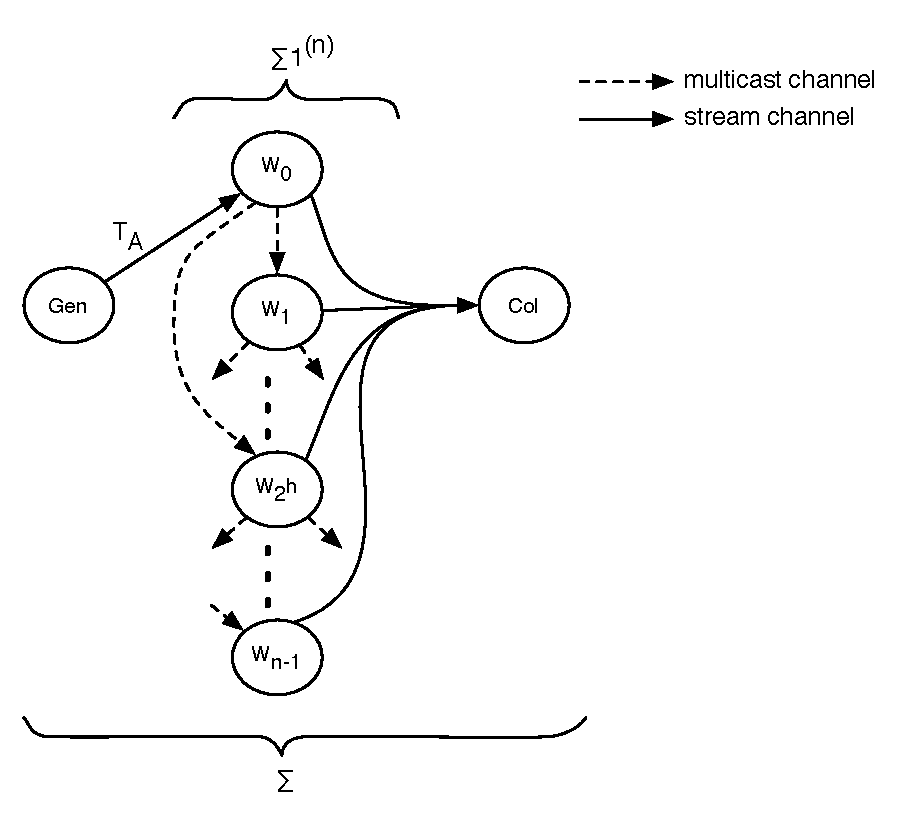
\includegraphics[scale=.5]{grafo_sigma.pdf}
  \caption[Computazione dell'implementazione parallela del benchmark]{Grafo della computazione Map (\subsystem) che \`e collegata allo stream e che fa uso della multicast strutturata ad albero binario mappato sull'insieme di processi worker}
  \label{fig:grafo_map}
\end{figure}
In questo modo, un worker, prima di avviare il proprio calcolo su un elemento dello stream prende parte alla comunicazione multicast dell'elemento stesso realizzata in modo distribuito sull'insieme dei worker. Questa soluzione (per un tempo di interarrivo superiore a 2 volte il tempo di servizio della multicast) permette di risparmiare nodi di elaborazione rispetto ad una soluzione con un sottosistema di nodi specializzato nella distribuzione multicast. 
Di contro, una realizzazione di questo tipo fa pagare il proprio tempo di servizio all'interno del tempo del sottosistema di calcolo nel caso in cui non sia possibile sovrapporre le comunicazioni al calcolo, come accade in \tile\ che non dispone dei supporti architetturali necessari nei PEs per l'esecuzione delle comunicazioni\footnote{Una forma di sovrapposizione esiste quando si fa uso del supporto alle comunicazioni che usa UDN, \`e infatti possibile che il trasferimento del messaggio sia eseguito in modo parzialmente sovrapposto all'esecuzione del calcolo del mittente.}.

La formulazione del tempo di servizio ideale e del grado di parallelismo ottimo del sottosistema Map differisce da quella definita precedentemente, in quanto occorre considerare che le comunicazioni non sono sovrapposte al calcolo. Di conseguenza nel tempo di servizio del sottosistema di calcolo si pagano completamente i tempi di servizio della multicast e della gather (equazione \ref{eq:impl_TsubsysId}), chiamiamo con \deltacom la somma di tali tempi. Anche il grado ottimo di parallelismo \`e rivalutato nella equazione \ref{eq:impl_nopt}.
\begin{flalign}
  \nonumber
  \inTsubsystemId \; &= \; \inTs \; 
  = \; \inTmult + \frac{\inTcalc}{n} + \inTgather \; \\ 
  \label{eq:impl_TsubsysId}
  &= \; 2 \cdot \inTsymsend + \frac{\inTcalc}{n} + \inTasyminsend \; 
  = \; \indeltacom + \frac{\inTcalc}{n} \\
  \label{eq:impl_nopt}
  n_{\mathrm{opt}} \; &= \; \left\lceil \frac{\inTcalc}{\inTa - \indeltacom} \right\rceil
\end{flalign}
Come ulteriore conseguenza, applicando la definizione di scalabilit\`a al tempo di servizio, non \`e possibile ottenere il valore ideale pari al grado di parallelismo usato.

\subsubsection{Sulla latenza di accesso alla memoria}
\label{sct:client_server}
I valori di \Tcalc, \deltacom(SM) e \deltacom(UDN) non sono costanti, ma variano con il  grado di parallelismo usato. All'aumentare del numero di processi coinvolti nell'applicazione aumentano il numero di richieste alla memoria condivisa e quindi aumenta l'uso delle reti di interconnessione e della gerarchia di memoria, con possibili congestioni, e in generale un aumento del tempo di risposta.
In particolare sia \Tcalc\ che $\indeltacom(\mathrm{SM})$ dipendono dalla latenza di accesso alla memoria e al sottosistema di cache, in quanto, in caso di \emph{fault} dei dati nella cache locale o nella cache home, \`e necessario trasferire il blocco corrispondente da un'altra cache o da un controllore di memoria, rispettivamente. Formalmente il problema pu\`o essere modellando come un sistema \emph{client-server}: un controllore di memoria, o una L2 cache, \`e considerato il modulo servente di un certo insieme di moduli clienti: il sottoinsieme dei PE che producono le richieste di accesso alla memoria a quel preciso modulo. Il tempo medio di risposta, $\Rq$, del servente \`e quindi caratterizzato dal periodo di tempo che la richiesta trascorre nella coda del servente, $\Wq$, pi\`u la latenza di elaborazione del servente. Essendo la computazione \emph{domanda e risposta} il fattore di utilizzazione $\rho$ del servente \`e sempre inferiore ad 1. Al variare del fattore di utilizzazione del servente il tempo di risposta $\Rq$ si mantiene pressocch\`e costante; dopo un certo valore, detto critico, di $\rho$, $\Rq$ aumenta asintoticamente ad infinito con $\rho$ che tende ad 1 (congestione). Il tempo di servizio effettivo di ogni cliente pu\`o essere caratterizzato dalla somma del tempo medio di calcolo pi\`u il $\Rq$. L'aumento della banda di richieste al servente, quindi l'aumento del fattore di utilizzazione $\rho$, e quindi l'aumento del tempo di risposta $\Rq$ pu\`o essere causato dalla riduzione del tempo (grana) di calcolo nei clienti, oppure dall'aumento del numero di clienti. In \cite{hpc_part2} \`e presentata una analisi della latenza di accesso alla memoria con e senza conflitti, e relativi modelli dei consti.
%% \begin{flalign}
%%   \inTcalc = \inTcalcId + \inTfault = \left [ \, \frac{\tau}{n}(1 + \theta) + \lambda \tau + \delta \, \right ] + \left [ \, \sum_i \inNfaulti \cdot \inTtrasfi  \, \right ]
%% \end{flalign}

\subsubsection{Descrizione dell'implementazione}
L'applicazione considerata \`e fittizia, ovvero non esiste un dispositivo, o processing element, che produce lo stream, come non esiste quello che lo riceve. Al fine di poter eseguire l'applicazione sono stati realizzati due processi, eseguiti in modo esclusivo su due PE della macchina, con il compito di produrre e consumare gli stream di matrici e di vettori rispettivamente. Questi processi sono collegati al sottosistema parallelo per mezzo dei canali messi a disposizione dal nostro supporto. Ne segue che il massimo parallelismo esplicitabile dalla macchina per la realizzazione della Map \`e $N = 59$, occorre infatti riservare un altro PE all'esecuzione del processo \verb+main+ dell'applicazione, e due PE sono riservati per l'esecuzione di funzionalit\`a del sistema operativo.

Il processo generatore dello stream \`e inizializzato con un tempo di interarrivo parametrico. La temporizzazione dello stream viene realizzata da questo processo invocando la primitiva di conteggio dei cicli di clock ed effettuando una attesa attiva sul valore del tempo trascorso, fin tanto che \`e minore al tempo di interarrivo specificato. Il processo generatore \`e collegato al primo processo worker del Map che costituisce il processo radice dell'albero che realizza la multicast. \`E compito di tale worker avviare la multicast distribuita sull'insieme dei worker per mezzo dei canali che costituiscono la struttura ad albero della comunicazione. Ogni processo worker \`e quindi collegato al processo collettore per mezzo di un canale asimmetrico in ingresso.

Il mapping dei processi nella macchina adottato consiste nell'eseguire i processi generatore e collettore nei primi due PE, i processi worker sono mappati in modo consecutivo a partire dal terzo PE, il processo main \`e mappato sull'ultimo PE disponibile. La topologia della comunicazione multicast si basa sull'applicazione della strategia \emph{depth-first} applicata al mapping di un albero binario nella sequenza lineare dei processi worker. 

L'applicazione \`e eseguita in modo parametrico nelle seguenti variabili:
\begin{itemize}
\item il tempo di interarrivo (\Ta) in cicli di clock,
\item la dimensione della matrice (il numero di righe M),
\item il grado di parallelismo del sottosistema Map ($n$),
\item la lunghezza dello stream ($m$), 
\item l'implementazione adottata dai canali simmetrici e dai canali asimmetrici in ingresso.
\end{itemize}
Si sono eseguite le misurazioni per due diverse configurazioni di implementazioni del supporto alle comunicazioni: utilizzando solo UDN, oppure solo la memoria condivisa. In tutte le esecuzioni si \`e adottata una lunghezza dello stream $m = 500$ sufficientemente maggiore al massimo grado di parallelismo esplicitabile (circa 60) affinch\`e sia possibile usare l'approssimazione dell'equazione \ref{eq:Tc}.

Le misure proposte nel seguito non sono mai relative ad una singola esecuzione, ma sono valori medi delle misure effettuate in un certo numero di esecuzioni sullo stesso tipo di computazione.

\subsubsection{Descrizione del metodo di misurazione}
Le misure prese in considerazione sono il tempo di completamento dello stream e il tempo di servizio del sottosistema Map. Tutti i processi dell'applicazione si sincronizzano su un oggetto di tipo barriera, il tempo di completamento viene avviato dopo che il processo generatore ha passato questa barriera e fermato al termine dell'esecuzione del processo collettore. Il tempo di servizio della Map \`e misurato nel processo worker alla radice dell'albero multicast ed \`e il risultato della media di tutti i tempi impiegati da tale processo tra la ricezione di due elementi contigui nello stream. 

Durante l'analisi saremo interessati a caratterizzare le presentazioni del sistema sotto altri punti di vista:
\begin{itemize}
\item il tempo di calcolo di un singolo prodotto scalare eseguito da un processo worker: per stimare questo valore viene misurato il tempo di calcolo di ogni singolo worker per ogni elemento dello stream, il tempo medio di calcolo viene quindi diviso per la dimensione della partizione (numero di righe). La misura \`e avviata in ogni worker dopo aver concluso la partecipazione alla multicast e viene conclusa prima di inviare il risultato al collettore.
\item il tempo di servizio della multicast: \`e stimato come media delle misure del tempo impiegato dal worker alla radice dell'albero mulitcast per eseguire l'invio ai due sotto-alberi.
\end{itemize}

\subsubsection{Risultati delle misurazioni}

Considerato che siamo interessati a computazioni di grana fine si sono considerare matrici con un numero di righe relativamente basso: $\mathrm{M} \in \{\,56, 168, 280\,\}$. Con il massimo grado di parallelismo, infatti, abbiamo partizioni di dimensione $g \in \{\,1, 3, 5\,\}$ righe, rispettivamente; conseguentemente, il calcolo svolto nei worker in tale situazione prevede $g\cdot\mathrm{M}$ moltiplicazioni e altrettante somme. Per ogni dimensione di matrice si sono eseguite istanze del programma di benchmark con grado di parallelismo della Map variabile. In ogni caso si \`e scelto $n$ divisore di $\mathrm{M}$.

Dato che non \`e imposto il tempo di interarrivo, si vorrebbe stimare il tempo di servizio della Map con il massimo numero di nodi disponibili, in modo tale da conoscere quale \`e la banda massima dello stream in cui il nostro sottosistema parallelo effettua il calcolo, producendo i risultati con la stessa velocit\`a. 
L'equazione da usare \`e quella mostrata precedentemente in formula~\ref{eq:impl_TsubsysId}. Se invece fosse noto il tempo di interarrivo dello stream, si userebbe l'equazione di formula~\ref{eq:impl_nopt} per ricavare il minimo numero di nodi worker necessari per eliminare il collo di bottiglia. Una previsione effettiva del comportamento del sistema stima i valori di \Tcalc\ e \deltacom per mezzo di simulazioni o applicando con modelli di costo formali che caratterizzano vari aspetti dell'architettura.

L'applicazione di modelli di costi all'architettura \tile\ non \`e lo scopo del tirocinio, si \`e quindi usato un approccio molto pi\`u semplice: \`e stimato in modo rudimentale il tempo di servizio ideale sostituendo nella formula~\ref{eq:impl_TsubsysId}, al  \Tcalc\ la misura del tempo di completamento effettuata sul programma sequenziale eseguito nella CPU di un singolo PE, e al \deltacom\ la misura della latenza di comunicazione descritta nell'esperimento precedente (sezione~\ref{sct:meter_risultati}).
Quello che otteniamo \`e una valutazione molto elementare del tempo di servizio che difficilmente sar\`a riscontrata nell'esecuzione del programma, perch\'e, ad esempio, non si \`e tenuto conto dell'aumento della latenza di accesso alla memoria con l'incremento del grado di parallelismo.
Nelle tabelle~\ref{tab:Tcalc},~\ref{tab:deltacom} sono riassunte le misure dei due parametri; in tabella~\ref{tab:TsubsysId} sono presentati i valori calcolati del tempo di servizio con il massimo grado di parallelismo ($N=59$). Il tempo di servizio effettivo del sistema viene mostrato nella sezione seguente.

\begin{table}[!h]
  \centering
  \begin{subtable}[b]{\textwidth}
    \centering
    \begin{tabular}{|r|r|r|}
      \hline
      \multicolumn{1}{ |c| }{ \multirow{2}{12ex}{\emph{Dimensione matrice}} } &
      \multicolumn{2}{ |c| }{ $\textrm{T}_{\textrm{calc}}$ } \\
      \cline{2-3}
      & $\tau$ & $\microsec$ \\
      \hline
      %% f = 864.583 Mhz 
      %% t = 1/864.583 microsec = 1.156626 nanosec    
      56x56  &  82934.927 &  95.924692 \\
      168x128 &  735319.293 & 850.489412 \\
      280x280 &  2040430.561 & 2360.015038\\
      \hline
    \end{tabular}
    \caption{Misurazioni del tempi di elaborazione del programma di calcolo sequenziale.}
    \label{tab:Tcalc}
  \end{subtable}

  \vspace{2ex}

  \begin{subtable}[b]{\textwidth}
    \centering
    \begin{tabular}{r|l|l|r|r|}
      \cline{2-5}
%      \multicolumn{1}{ |c| }{ \multirow{2}{*}{\emph{Implementazione usata}} } & 
      & \multicolumn{2}{ |c| }{ \emph{Implementazione usata}} & 
      \multicolumn{2}{ |c| }{ $\indeltacom$ } \\
      \cline{2-5}
      & \emph{canale simmetrico} & \emph{canale asimmetrico} & $\tau$ & $\microsec$ \\
      \cline{2-5}
      {\footnotesize UDN} & \verb+ch_sym_udn+ & \verb+ch_asymin_udn+ & 180.95523 & 0.20929 \\
      & \verb+ch_sym_sm+ & \verb+ch_asymin_sm+ & 481.04016 & 0.55638 \\
      {\footnotesize SM} & \verb+ch_sym_sm+ & \verb+ch_asymin_sm_all+ & 724.91273 & 0.83845 \\
      %% \verb+udn+ & \verb+udn+ & 180.95523 & 0.20929 \\
      %% \verb+sm+ & \verb+sm+ & 481.04016 & 0.55638 \\
      %% \verb+sm+ & \verb+sm_all+ & 724.91273 & 0.83845 \\
      \cline{2-5}
    \end{tabular}
    \caption{Stima di \deltacom\ per mezzo delle misure della latenza dei canali effettuate in sezione~\ref{sct:meter_risultati} con i due processi distanti 14 hops.}
    \label{tab:deltacom}
  \end{subtable}

  \vspace{2ex}

  \begin{subtable}[b]{\textwidth}
    \centering
    \begin{tabular}{|r|r|r|r|r|}
      \hline
      \multicolumn{1}{ |c| }{ \multirow{2}{*}{M} } & 
      \multicolumn{2}{ |c| }{ $\inTsubsystemId$(UDN) } &
      \multicolumn{2}{ |c| }{ $\inTsubsystem$(SM) } \\[2pt] 
      \cline{2-5}
      & $\tau$ & $\mu\mathrm{sec}$ 
      & $\tau$ & $\mu\mathrm{sec}$ \\
      \hline
      56 & 1586.632 & 1.835 & 2130.589 & 2.464 \\
      168 & 12643.994 & 14.624 & 13187.952 & 15.254 \\
      280 & 34764.524 & 40.210 & 35308.482 & 40.839 \\
      %% 56 & 1408.7445 & 1.6293905421 \\
      %% 168 & 12466.1066 & 14.41862307 \\
      %% 280 & 34586.6366 & 40.00380317\\
      \hline
    \end{tabular}
    \caption{Valori del tempo di servizio ideali della Map con grado di parallelismo massimo ($N=59$). Sono ottenuti sostituendo i valori delle tabelle~\ref{tab:Tcalc},~\ref{tab:deltacom} alla formula~\ref{eq:impl_TsubsysId}.}
    \label{tab:TsubsysId}
  \end{subtable}

%% \caption{Valori ideali dei tempi di calcolo e di comunicazione}
  \caption[Tempi di servizio ideali del benchmark]{}
  \label{tab:Tcalc_deltacom_TsubsysId}
\end{table}


%% 09061135
%% \begin{table}[p]
%%   \centering
%%   \begin{subtable}[b]{\textwidth}
%%     \centering
%%     \begin{tabular}{|l|c|c|}
%%       \hline
%%       \emph{Matrix Size} & $\textrm{T}_{\textrm{calc}} \, (\,\tau\,)$ & $\textrm{T}_{\textrm{calc}} \, (\,\microsec\,)$ \\[2pt]
%%       \hline
%%       %% f = 864.583 Mhz 
%%       %% t = 1/864.583 microsec = 1.156626 nanosec    
%%       56x56  &  82934.927 &  95.924692 \\
%%       168x128 &  735319.293 & 850.489412 \\
%%       280x280 &  2040430.561 & 2360.015038\\
%%       \hline
%%     \end{tabular}
%%     \caption{Misurazioni del tempi di elaborazione del programma di calcolo sequenziale.}
%%     \label{tab:Tcalc}
%%   \end{subtable}

%%   \vspace{2ex}

%%   \begin{subtable}[b]{\textwidth}
%%     \centering
%%     \begin{tabular}{|l|r|r|}
%%       \hline
%%       \emph{Canali usati} & $\indeltacom \, (\,\tau\,)$ & $\indeltacom \, (\,\microsec\,)$ \\[2pt]
%%       \hline
%%       UDN only & 180.95523 & 0.20929 \\
%%       SM only & 481.04016 & 0.55638 \\
%%       SM only, with all senders  & 724.91273 & 0.83845 \\
%%       \hline
%%     \end{tabular}
%%     \caption{Valori ideali della somma dei tempi impiegati nelle comunicazioni dai processi worker della Map (misure con \#hops = 14).}
%%     \label{tab:deltacom}
%%   \end{subtable}

%%   \vspace{2ex}

%%   \begin{subtable}[b]{\textwidth}
%%     \centering
%%     \begin{tabular}{|l|l|l|}
%%       \hline
%%       M & $\inTsubsystemId (\,\tau\,)$ & $\inTsubsystemId (\,\mu \mathrm{sec}\,)$ \\[2pt]
%%       \hline
%%       56 & 1408.7445225254237 & 1.6293905421104913 \\
%%       168 & 12466.106655644067 & 14.418623076690981 \\
%%       280 & 34586.636626711865 & 40.003803175007249 \\
%%       \hline
%%     \end{tabular}
%%     \caption{Valori del tempo di servizio ideale della Map con grado di parallelismo massimo ($N=59$)}
%%     \label{tab:TsubsysId}
%%   \end{subtable}

%% %% \caption{Valori ideali dei tempi di calcolo e di comunicazione}
%%   \caption{}
%%   \label{tab:Tcalc_deltacom_TsubsysId}
%% \end{table}



\FloatBarrier

\subsubsection*{Misura dei tempi di completamento e di servizio al variare del tempo di ingresso}
Si sono sperimentate pi\`u esecuzioni dell'applicazione con diversi valori del tempo di interarrivo dello stream: 
\begin{enumerate}  
\item viene considerata una banda di arrivi per la quale non si riesce ad eliminare il collo di bottiglia; in particolare questo esperimento ci mostra qual'\`e il tempo di servizio effettivo che assume il sottosistema;
\item Una volta noto il tempo di servizio effettivo si considerano velocit\`a degli arrivi superiori a questo valore, per i quali deve essere eliminato il collo di bottiglia. Scopo di questi esperimenti \`e verificare che il collo di bottiglia sia effettivamente eliminato, e con che grado di parallelismo $n$ si riesce ad eliminare, in particolare se il valore di questo $n$ \`e vicino a quello stimato con la formula~\ref{eq:impl_nopt}.
%% scopo di questi esperimenti \`e verificare tale comportamento del sistema ed accertarsi che la scalabilit\`a del tempo di servizio sia simile al grado di parallelismo ottimo calcolato con la formula~\ref{eq:impl_nopt}.
\end{enumerate}     
I risultati degli esperimenti fatti sono mostrati in figura~\ref{fig:serviceTime} per quanto riguarda il tempo di servizio della Map, e in figura~\ref{fig:completeTime} per il tempo di completamento dello stream. La scalabilit\`a \`e calcolata con la formula~\ref{eq:s} sostituendo al tempo di calcolo, quello misurato sul programma sequenziale e presentato in tabella~\ref{tab:Tcalc}. I grafici di scalabilit\`a sono quindi mostrati in figura~\ref{fig:completeTimeScalability}. Si ricorda che il tempo di servizio effettivo della Map \`e il massimo tra il tempo di interarrivo e il tempo di servizio ideale, costituito, quest'ultimo, dal tempo di calcolo sulla partizione della matrice, pi\`u \deltacom\ il tempo speso nelle comunicazioni. Per un generico tempo di interarrivo abbiamo due possibili soluzioni:
\begin{description}   
\item [la Map \`e collo di bottiglia:] \`e interessante verificare quale sia il tempo di interarrivo effettivo della Map, e di conseguenza la massima scalabilit\`a effettiva della Map. In precedenza si \`e infatti osservato che le formule usate per stimare il tempo di servizio della Map non applicano alcun modello dei costi relativo ad aspetti dell'architettura, ma si limitano ad usare le misure su computazioni particolari. In seguito ai conflitti sulle reti di interconnessione e sui sottosistemi della gerarchia di memoria si prevede un aumento del tempo di calcolo nei worker, rispetto a $\frac{\inTcalc}{n}$, e un aumento della latenza di comunicazione, rispetto a quella misurata. Applicando la formula del $n_{\mathrm{opt}}$ ai valori effettivi del tempo di calcolo e della latenza di comunicazione si ottiene un valore maggiore rispetto a quello stimato inizialmente. 
%Allo stesso modo si trova un valore di tempo di servizio ideale maggiore. 
La tabella~\ref{tab:scalability_serviceTime_bottleneck} mostra i tempi di servizio effettivi, per le varie dimensioni delle matrici. Questi sono molto superiori ai tempi di servizio ideali relativi al massimo $n$ esplicitabile (59), mostrati in tabella~\ref{tab:TsubsysId}.

%% in questo caso si valuta la scalabilit\`a come 
%%   \[ \inscal = \frac{\inTcalc}{\frac{\inTcalc}{n} + \indeltacom} \]
%%   La tabella~\ref{tab:scalability_serviceTime_bottleneck} propone il miglior tempo di servizio per le esecuzioni del programma in cui la Map \`e collo di bottiglia. Tale valore \`e il minimo tempo di servizio raggiungibile: una qualsiasi altra esecuzione con tempo di interarrivo inferiore fornisce gli stessi risultati di tempo di servizio del sistema.

\item [la Map non \`e collo di bottiglia:] esiste un certo grado di parallelismo, esplicitabile dalla macchina, per cui il tempo di servizio ideale della Map \`e inferiore al tempo di interarrivo. Indipendentemente da un ulteriore aumento di $n$, il tempo di servizio effettivo del sistema rimane costante al tempo di interarrivo e la scalabilit\`a rimane sempre uguale al grado di parallelismo ottimo. \`E possibile che con l'aumentare del grado di parallelismo si creino delle degradazioni per cui il tempo di interarrivo e la scalabilit\`a diminuiscono leggermente rispetto a quelli dell'$n$ ottimo. 

Le misure effettuate mostrano che il tempo di servizio effettivo del sistema raggiunge il tempo di interarrivo con un valore di $n$ ``vicino a quello ottimo''. Stesso ragionamento si applica alla scalabilit\`a, la quale raggiunge il valore ottimo di $n$ con un grado di parallelismo vicino a questo valore. I valori misurati per alcuni tempi di interarrivo sono mostrati nella tabella~\ref{tab:scalability_serviceTime_noBottleneck}. Il comportamento del sistema \`e quindi quello atteso. Si osserva inoltre che la stima del grado di parallelismo ottimo \`e tanto migliore quanto la dimensione della matrice \`e pi\`u grande.
%% Tale situazione risulta verificata nelle misure degli esperimenti, con tempi di interarrivo elevati, in tabella~\ref{tab:scalability_serviceTime_noBottleneck} sono mostrati i migliori tempi di servizio, e corrispondente scalablit\`a e grado di parallelismo usato, quando la Map non \`e collo di bottiglia.
\end{description}      

%\cellcolor[gray]
\definecolor{Gray}{gray}{0.9}
\newcommand{\clr}{\cellcolor[gray]{0.9}}


\renewcommand{\arraystretch}{1.5}

\begin{table}[p]
  \begin{tabular}{|r|c|r||r||r|r|r|}
    \hline
    M & \Ta & \emph{Impl} & $n_{\mathrm{opt}}$ & $n$ & $\inscal$ & $\inTsubsystem (\tau)$ \\[2pt]
    \hline
    \multirow{2}{*}{56} & \multirow{2}{*}{$4\cdot10^3$ $\tau$ = 4.626 $\microsec$} 
    & UDN & 21.716     & 56 & 15.529 & 5340.578  \\
    \cline{3-7}
    & & SM & 23.568     & 28 & 10.982 & 7552.140  \\
    \hline
    \multirow{2}{*}{168} & \multirow{2}{*}{$20\cdot10^3$ $\tau$ = 23.1325 $\microsec$} 
    & UDN & 37.102     & 56 & 33.894 & 21694.473  \\
    \cline{3-7}
    & & SM & 37.672     & 56  & 30.582 & 24044.160 \\
    \hline
    \multirow{2}{*}{280} & \multirow{2}{*}{$50\cdot10^3$ $\tau$ = 57.831 $\microsec$} 
    & UDN & 40.957     & 56  & 37.495 & 54419.290 \\
    \cline{3-7}
    & & SM & 41.205     & 56 & 36.937  & 55241.196 \\
    \hline
  \end{tabular}
  \caption{Tempi di servizio effettivo e scalabilit\`a della Map \emph{migliori} quando la Map \`e collo di bottiglia.}
  \label{tab:scalability_serviceTime_bottleneck}
\end{table}

\renewcommand{\arraystretch}{1.2}

\begin{table}[p]
  \begin{tabular}{|r|c|r||r||r|r|r|}
    \hline
    M & \Ta & \emph{Impl} & $n_{\mathrm{opt}}$ & $n$ & $\inscal$ & $\inTsubsystem (\tau)$ \\[2pt]
    \hline
    \multirow{4}{*}{56} & \multirow{4}{*}{$10\cdot10^3$ $\tau$ = 11.566 $\microsec$} 
    %14 10089.544800 10133.046000 10031.912000 32.730468 8.219888 0.121656 0.011670 11.669830
    & \multirow{2}{*}{UDN} &  \multirow{2}{*}{8.446}
    & 8 & 7.074 & 11723.431 \\
    & & & & \clr 14 & \clr 8.220 & \clr 10089.545 \\
    \cline{3-7}
    & & \multirow{2}{*}{SM} & \multirow{2}{*}{8.713}
    & 8 & 6.491 & 12776.486 \\
    & & & & \clr 14 & \clr 8.182 & \clr 10136.235 \\
    \hline
    \multirow{4}{*}{168} & \multirow{4}{*}{$50\cdot10^3$ $\tau$ = 57.831 $\microsec$} 
    & \multirow{2}{*}{UDN} & \multirow{2}{*}{14.718}
    & 14 & 13.336 & 55139.259 \\
    & & & & \clr 21 & \clr 14.739 & \clr 49888.153 \\
    %      & & & & \clr 28 & \clr 14.741 & \clr 49882.893 \\
    \cline{3-7}
    & & \multirow{2}{*}{SM} & \multirow{2}{*}{14.807}
    & 14 & 13.095 & 56151.886 \\
    & & & & \clr 21 & \clr 14.735 & \clr 49902.936 \\
    %      & & & & \clr 24 & \clr 14.740 & \clr 49885.909 \\
    \hline
    \multirow{4}{*}{280} & \multirow{4}{*}{$10\cdot10^4$ $\tau$ = 115.662 $\microsec$} 
    & \multirow{2}{*}{UDN} & \multirow{2}{*}{20.441}
    & 20 & 20.433 & 99859.243 \\
    & & & & \clr 28 & \clr 20.448 & \clr 99787.616 \\
    %      & & & & \clr 40 & \clr 20.448 & \clr 99786.505 \\
    \cline{3-7}
    & & \multirow{2}{*}{SM} & \multirow{2}{*}{20.503}
    & 20 & 20.163 & 101196.684 \\
    & & & & \clr 28 & \clr 20.450 & \clr 99778.438 \\
    \hline
  \end{tabular}
  \caption{Tempi di servizio effettivo e scalabilit\`a della Map quando la Map non \`e collo di bottiglia. Vengono mostrati i valori relativi al grado di parallelismo vicino al valore ottimo calcolato.}
  \label{tab:scalability_serviceTime_noBottleneck}
\end{table}
%% \caption[Tempi di servizio effettivi del benchmark]{Vengono proposti i migliori tempi di servizio, con relativo grado di parallelismo, per due tipologie di tempi di interarrivo: quelli nel quale la Map \`e collo di bottiglia, e quelli in cui la Map non \`e collo di bottiglia.}
%% \label{tab:scalability_serviceTime}

\renewcommand{\arraystretch}{1}

%% \begin{table}[!h]
%%   \begin{tabular}{|c|r||r||r|r|r|}
%%     \hline
%%     M, \Ta & \emph{Impl} & $n_{\mathrm{opt}}$ & $n$ & $\inscal$ & $\inTsubsystem (\tau)$ \\[2pt]
%%     \hline
%%     \multirow{2}{*}{56, 4000 $\tau$ = 4.626 $\microsec$} 
%%     & UDN & 21.716     & 56 & 15.037 & 5340.578  \\
%%     \cline{2-6}
%%     & SM & 23.568     & 28 & 10.660 & 7552.140  \\
%%     \hline
%%     \multirow{2}{*}{168, 20000 $\tau$ = 23.1325 $\microsec$} 
%%     & UDN & 37.102     & 56 & 33.338 & 21694.473  \\
%%     \cline{2-6}
%%     & SM & 37.672     & 56  & 30.098 & 24044.160 \\
%%     \hline
%%     \multirow{2}{*}{280, 50000 $\tau$ = 57.831 $\microsec$} 
%%     & UDN & 40.957     & 56  & 37.188 & 54419.290 \\
%%     \cline{2-6}
%%     & SM & 41.205     & 56 & 36.644  & 55241.196 \\
%%     \hline
%%     \hline
%%     \multirow{2}{*}{56, 10000 $\tau$ = 11.566 $\microsec$} 
%%     & UDN &  8.446     & 14 & 8.220 & 10089.545 \\
%%     \cline{2-6}
%%     & SM & 8.713      & 14 & 8.182 & 10136.235 \\
%%     \hline
%%     \multirow{2}{*}{168, 50000 $\tau$ = 57.831 $\microsec$} 
%%     & UDN & 14.718     & 28 & 14.741 & 49882.893 \\
%%     \cline{2-6}
%%     & SM & 14.807      & 24 & 14.740 & 49885.909 \\
%%     \hline
%%     \multirow{2}{*}{280, 100000 $\tau$ = 115.662 $\microsec$} 
%%     & UDN & 20.441     & 40 & 20.448 & 99786.505 \\
%%     \cline{2-6}
%%     & SM & 20.503     & 28 & 20.450 & 99778.438 \\
%%     \hline
%%   \end{tabular}
%% \end{table}


\FloatBarrier

\begin{figure}[p]
  \caption[Tempi di servizio del sottosistema Map]{Grafici del tempo di servizio del sottosistema Map al variare del tempo di interarrivo}
  \begin{subfigure}[b]{.5\columnwidth}
    \centering
    \renewcommand\thesubfigure{\alph{subfigure}}
    %% se vuoi spostare questa caption in fondo devi modificare anche i contatori!
    \caption{Utilizzo del supporto su UDN}
    \begin{subfigure}[b]{\textwidth}
      \centering
      \addtocounter{subfigure}{-1}
      \renewcommand\thesubfigure{\alph{subfigure}1}
      \resizebox{\columnwidth}{!}{\input{plot-T-millis_nogatherInt_00_500_selected_56.tex}}
      \caption{Dimensione della matrice 56x56}
      \label{fig:serviceTime_UDN_size56}
    \end{subfigure}
    ~
    \begin{subfigure}[b]{\textwidth}
      \centering
      \addtocounter{subfigure}{-1}
      \renewcommand\thesubfigure{\alph{subfigure}2}
      \resizebox{\columnwidth}{!}{\input{plot-T-millis_nogatherInt_00_500_selected_168.tex}}
      \caption{Dimensione della matrice 168x168}
      \label{fig:serviceTime_UDN_size168}
    \end{subfigure}
    ~
    \begin{subfigure}[b]{\textwidth}
      \centering
      \addtocounter{subfigure}{-1}
      \renewcommand\thesubfigure{\alph{subfigure}3}
      \resizebox{\columnwidth}{!}{\input{plot-T-millis_nogatherInt_00_500_selected_280.tex}}
      \caption{Dimensione della matrice 280x280}
      \label{fig:serviceTime_UDN_size280}
    \end{subfigure}
    \label{fig:serviceTime_UDN}
  \end{subfigure}
  \hspace{2ex}
  \begin{subfigure}[b]{.5\columnwidth}
    \centering
    \renewcommand\thesubfigure{\alph{subfigure}}
    \caption{Utilizzo del supporto sulla SM}
    \begin{subfigure}[b]{\textwidth}
      \centering
      \addtocounter{subfigure}{-1}
      \renewcommand\thesubfigure{\alph{subfigure}1}
      \resizebox{\columnwidth}{!}{\input{plot-T-millis_nogatherInt_11_500_selected_56.tex}}
      \caption{Dimensione della matrice 56x56}
      \label{fig:serviceTime_SM_size56}
    \end{subfigure}
    ~
    \begin{subfigure}[b]{\textwidth}
      \centering
      \addtocounter{subfigure}{-1}
      \renewcommand\thesubfigure{\alph{subfigure}2}
      \resizebox{\columnwidth}{!}{\input{plot-T-millis_nogatherInt_11_500_selected_168.tex}}
      \caption{Dimensione della matrice 168x168}
      \label{fig:serviceTime_SM_size168}
    \end{subfigure}
    ~
    \begin{subfigure}[b]{\textwidth}
      \centering
      \addtocounter{subfigure}{-1}
      \renewcommand\thesubfigure{\alph{subfigure}3}
      \resizebox{\columnwidth}{!}{\input{plot-T-millis_nogatherInt_11_500_selected_280.tex}}
      \caption{Dimensione della matrice 280x280}
      \label{fig:serviceTime_SM_size280}
    \end{subfigure}
    \label{fig:serviceTime_SM}
  \end{subfigure}
  \label{fig:serviceTime}
\end{figure}


\begin{figure}[p]
  \caption[Tempi di completamento dello stream]{Grafici del tempo di completamento dello stream al variare del tempo di interarrivo}
  \begin{subfigure}[b]{.5\columnwidth}
    \centering
    \renewcommand\thesubfigure{\alph{subfigure}}
    %% se vuoi spostare questa caption in fondo devi modificare anche i contatori!
    \caption{Utilizzo del supporto su UDN}
    \begin{subfigure}[b]{\textwidth}
      \centering
      \addtocounter{subfigure}{-1}
      \renewcommand\thesubfigure{\alph{subfigure}1}
      \resizebox{\columnwidth}{!}{\input{plot-Tc_nogatherInt_00_500_selected_56.tex}}
      \caption{Dimensione della matrice 56x56}
      \label{fig:completeTime_UDN_size56}
    \end{subfigure}
    ~
    \begin{subfigure}[b]{\textwidth}
      \centering
      \addtocounter{subfigure}{-1}
      \renewcommand\thesubfigure{\alph{subfigure}2}
      \resizebox{\columnwidth}{!}{\input{plot-Tc_nogatherInt_00_500_selected_168.tex}}
      \caption{Dimensione della matrice 168x168}
      \label{fig:completeTime_UDN_size168}
    \end{subfigure}
    ~
    \begin{subfigure}[b]{\textwidth}
      \centering
      \addtocounter{subfigure}{-1}
      \renewcommand\thesubfigure{\alph{subfigure}3}
      \resizebox{\columnwidth}{!}{\input{plot-Tc_nogatherInt_00_500_selected_280.tex}}
      \caption{Dimensione della matrice 280x280}
      \label{fig:completeTime_UDN_size280}
    \end{subfigure}
    \label{fig:allScalbility_UDN}
  \end{subfigure}
  \hspace{2ex}
  \begin{subfigure}[b]{.5\columnwidth}
    \centering
    \renewcommand\thesubfigure{\alph{subfigure}}
    \caption{Utilizzo del supporto sulla SM}
    \begin{subfigure}[b]{\textwidth}
      \centering
      \addtocounter{subfigure}{-1}
      \renewcommand\thesubfigure{\alph{subfigure}1}
      \resizebox{\columnwidth}{!}{\input{plot-Tc_nogatherInt_11_500_selected_56.tex}}
      \caption{Dimensione della matrice 56x56}
      \label{fig:completeTime_SM_size56}
    \end{subfigure}
    ~
    \begin{subfigure}[b]{\textwidth}
      \centering
      \addtocounter{subfigure}{-1}
      \renewcommand\thesubfigure{\alph{subfigure}2}
      \resizebox{\columnwidth}{!}{\input{plot-Tc_nogatherInt_11_500_selected_168.tex}}
      \caption{Dimensione della matrice 168x168}
      \label{fig:completeTime_SM_size168}
    \end{subfigure}
    ~
    \begin{subfigure}[b]{\textwidth}
      \centering
      \addtocounter{subfigure}{-1}
      \renewcommand\thesubfigure{\alph{subfigure}3}
      \resizebox{\columnwidth}{!}{\input{plot-Tc_nogatherInt_11_500_selected_280.tex}}
      \caption{Dimensione della matrice 280x280}
      \label{fig:completeTime_SM_size280}
    \end{subfigure}
    \label{fig:allcompleteTime_SM}
  \end{subfigure}
  \label{fig:completeTime}
\end{figure}

\begin{figure}[p]
  \caption[Scalabilit\`a del tempo di completamento]{Grafici di scalabilit\`a del tempo di completamento dello stream al variare del tempo di interarrivo}
  \begin{subfigure}[b]{.5\columnwidth}
    \centering
    \renewcommand\thesubfigure{\alph{subfigure}}
    %% se vuoi spostare questa caption in fondo devi modificare anche i contatori!
    \caption{Utilizzo del supporto su UDN}
    \begin{subfigure}[b]{\textwidth}
      \centering
      \addtocounter{subfigure}{-1}
      \renewcommand\thesubfigure{\alph{subfigure}1}
      \resizebox{\columnwidth}{!}{\input{plot-Tc-s_nogatherInt_00_500_selected_56.tex}}
      \caption{Dimensione della matrice 56x56}
      \label{fig:completeTimeScalabilityTc_UDN_size56}
    \end{subfigure}
    ~
    \begin{subfigure}[b]{\textwidth}
      \centering
      \addtocounter{subfigure}{-1}
      \renewcommand\thesubfigure{\alph{subfigure}2}
      \resizebox{\columnwidth}{!}{\input{plot-Tc-s_nogatherInt_00_500_selected_168.tex}}
      \caption{Dimensione della matrice 168x168}
      \label{fig:completeTimeScalabilityTc_UDN_size168}
    \end{subfigure}
    ~
    \begin{subfigure}[b]{\textwidth}
      \centering
      \addtocounter{subfigure}{-1}
      \renewcommand\thesubfigure{\alph{subfigure}3}
      \resizebox{\columnwidth}{!}{\input{plot-Tc-s_nogatherInt_00_500_selected_280.tex}}
      \caption{Dimensione della matrice 280x280}
      \label{fig:completeTimeScalabilityTc_UDN_size280}
    \end{subfigure}
    \label{fig:completeTimeScalabilityTc_UDN}
  \end{subfigure}
  \hspace{2ex}
  \begin{subfigure}[b]{.5\columnwidth}
    \centering
    \renewcommand\thesubfigure{\alph{subfigure}}
    \caption{Utilizzo del supporto sulla SM}
    \begin{subfigure}[b]{\textwidth}
      \centering
      \addtocounter{subfigure}{-1}
      \renewcommand\thesubfigure{\alph{subfigure}1}
      \resizebox{\columnwidth}{!}{\input{plot-Tc-s_nogatherInt_11_500_selected_56.tex}}
      \caption{Dimensione della matrice 56x56}
      \label{fig:completeTimeScalabilityTc_SM_size56}
    \end{subfigure}
    ~
    \begin{subfigure}[b]{\textwidth}
      \centering
      \addtocounter{subfigure}{-1}
      \renewcommand\thesubfigure{\alph{subfigure}2}
      \resizebox{\columnwidth}{!}{\input{plot-Tc-s_nogatherInt_11_500_selected_168.tex}}
      \caption{Dimensione della matrice 168x168}
      \label{fig:completeTimeScalabilityTc_SM_size168}
    \end{subfigure}
    ~
    \begin{subfigure}[b]{\textwidth}
      \centering
      \addtocounter{subfigure}{-1}
      \renewcommand\thesubfigure{\alph{subfigure}3}
      \resizebox{\columnwidth}{!}{\input{plot-Tc-s_nogatherInt_11_500_selected_280.tex}}
      \caption{Dimensione della matrice 280x280}
      \label{fig:completeTimeScalabilityTc_SM_size280}
    \end{subfigure}
    \label{fig:completeTimeScalabilityTc_SM}
  \end{subfigure}
  \label{fig:completeTimeScalability}
\end{figure}



\FloatBarrier

\subsubsection*{Analisi delle possibili degradazioni}
Si \`e indagato su quali siano le cause della cattiva scalabilit\`a che caratterizzano le esecuzioni, in particolar modo quella con dimensione minore dei dati. Esiste una parte, o pi\`u parti, del sistema che non si comporta come descritto dalla formula applicata per calcolare la scalabilit\`a. 
  Il sistema pu\`o essere visto come costituito da tre fasi collegate in pipeline: multicast, calcolo, gather. Il programma \`e stato rieseguito misurando il tempo di servizio di ciascuna fase, al fine di verificare il comportamento effettivo del sistema. Da tali misurazioni non risulta problematica la fase di gathering, mentre sono le altre due fasi che aumentano il proprio tempo di servizio con il crescere di $n$. 
\begin{description}
\item [fase di calcolo] le misure del tempo di calcolo sono proposte in maniera leggermente elaborata nelle figura~\ref{fig:rowTime_int}: viene esposto il rapporto tra i tempi di calcolo di un singolo prodotto scalare nel programma sequenziale e nel calcolo di un worker del sistema parallelo di grado $n$. Tale rapporto dovrebbe essere costante, indipendentemente dal grado di parallelismo; si osserva tuttavia un aumento di tale rapporto al crescere di $n$. Questa degradazione \`e tanto maggiore quanto pi\`u piccole sono le dimensioni dei dati. \`E ragionevole ipotizzare la causa di questo comportamento come l'aumento del tempo di risposta alla memoria indotto dall'incremento del numero di richieste alla memoria prodotto da valori crescenti di $n$. Come spiegato precedentemente, l'aumento del numero di clienti in una computazione \emph{client-server domanda-e-risposta} produce un aumento del tempo di risposta medio del servente. Inoltre il fatto che la degradazione sia maggiore con dimensione pi\`u piccola della matrice porta a convincersi di tale ragionamento, in quanto la diminuzione della dimensione dei dati porta ad un calo della grana di computazione dei worker, e quindi ad un aumento della frequenza di accessi alla memoria (controllore o L2 cache home) dovuti al verificarsi di un fault nella cache locale. Per convincersi di tale ragionamento, e grazie ad una particolare caratteristica architetturale, \`e stato effettuato un ulteriore esperimento, mostrato in figura~\ref{fig:rowTime_float}: la stessa misurazione \`e presa per dati in virgola mobile.  I core di \tile\ non dispongono di unit\`a di elaborazione firmware per i calcoli in virgola mobile, pertanto tali conti vengono interpretati a livello assembler. Ne segue che un calcolo aritmetico in virgola mobile viene interpretato come molte istruzioni assembler. Rispetto allo stesso calcolo con tipi interi, si ha una frequenza di accesso alla memoria inferiore, con conseguente riduzione del tempo di risposta. Il comportamento mostrato dall'esperimento con dati float ha infatti il tempo di calcolo del singolo prodotto scalare costante (o quasi) per tutte le dimensioni della matrice.
\item [fase di multicast] dato che la multicast non \`e realizzata da un sottosistema distinto da quello di calcolo, ma \`e mappata nei worker, si sono considerati i tempi di servizio della multicast relativi alle situazioni in cui il sistema non \`e collo di bottiglia. Le misurazioni sono mostrate in figura~\ref{fig:multicast}. I valori effettivi delle comunicazioni, in una applicazione \emph{reale}, risultano maggiori rispetto a quelli misurati con l'applicazione ping-pong. Si osserva inoltre un aumento del tempo di servizio con l'aumentare di $n$, soprattutto con dimensioni piccole dei dati. Anche in questo caso, tale tempo di servizio sarebbe dovuto essere costante. Per il supporto che usa la memoria condivisa possono essere portate le stesse argomentazioni della fase di calcolo.
\end{description}

\begin{figure}[!b]
  \caption[Aumento del tempo di calcolo di un singolo prodotto scalare]{Fattore di variazione del tempo di calcolo di un singolo prodotto scalare: rapporto tra il tempo medio di calcolo di un singolo prodotto scalare nel calcolo di un worker della Map rispetto allo stesso tempo nel programma sequenziale. La Map \`e collo di bottiglia: $\inTa = 4.626 \microsec$.}
  \begin{subfigure}[b]{.5\textwidth}
    \centering
    \renewcommand\thesubfigure{\alph{subfigure}}
    \caption{Utilizzo di dati di tipo Intero}
    \begin{subfigure}[b]{\textwidth}
      \centering
      \addtocounter{subfigure}{-1}
      \renewcommand\thesubfigure{\alph{subfigure}1}
      \resizebox{\columnwidth}{!}{\input{plot-rowCalcT_nogatherInt_00_500_4000_all.tex}}
      \caption{Utilizzo del supporto su UDN}
      \label{fig:rowTime_int_udn}
    \end{subfigure}
    ~
    \begin{subfigure}[b]{\textwidth}
      \addtocounter{subfigure}{-1}
      \renewcommand\thesubfigure{\alph{subfigure}2}
      \resizebox{\columnwidth}{!}{\input{plot-rowCalcT_nogatherInt_11_500_4000_all.tex}}
      \caption{Utilizzo del supporto su SM}
      \label{fig:rowTime_int_sm}
    \end{subfigure}
    \label{fig:rowTime_int}
  \end{subfigure}
  %%%%%%%%%%%%%%%%%%%%%%%%%%%%%%
  \hspace{2ex}
  %%%%%%%%%%%%%%%%%%%%%%%%%%%%%%
  \begin{subfigure}[b]{.5\textwidth}
    \centering
    \renewcommand\thesubfigure{\alph{subfigure}}
    \caption{Utilizzo di dati di tipo Floating Point}
    \begin{subfigure}[b]{\textwidth}
      \centering
      \addtocounter{subfigure}{-1}
      \renewcommand\thesubfigure{\alph{subfigure}1}
      \resizebox{\columnwidth}{!}{\input{plot-rowCalcT_nogatherFloat_00_500_4000_all.tex}}
      \caption{Utilizzo del supporto su UDN}
    \end{subfigure}
    ~
    \begin{subfigure}[b]{\textwidth}
      \centering
      \addtocounter{subfigure}{-1}
      \renewcommand\thesubfigure{\alph{subfigure}2}
      \resizebox{\columnwidth}{!}{\input{plot-rowCalcT_nogatherFloat_11_500_4000_all.tex}}
      \caption{Utilizzo del supporto su SM}
    \end{subfigure}
    \label{fig:rowTime_float}
  \end{subfigure}
  \label{fig:rowTime}
\end{figure}

%% 6 GRAFICI DEL TEMPO DI SERVIZIO DELLA MULTICAST QUANDO LA MAP NON E` COLLO DI BOTTIGLIA. VARIA TA PER DIMENSIONE DATI FISSA PER UDN E PER SM
%% POCO SIGNIFICATIVO
%% \begin{figure}[p]
%%   \caption{Grafici del tempo di multicast al variare del tempo di interarrivo}
%%   \begin{subfigure}[b]{.5\columnwidth}
%%     \centering
%%     \renewcommand\thesubfigure{\alph{subfigure}}
%%     %% se vuoi spostare questa caption in fondo devi modificare anche i contatori!
%%     \caption{Implementazione con solo UDN}
%%     \begin{subfigure}[b]{\textwidth}
%%       \centering
%%       \addtocounter{subfigure}{-1}
%%       \renewcommand\thesubfigure{\alph{subfigure}1}
%%       \resizebox{\columnwidth}{!}{\input{plot-Tmult-nb_nogatherInt_00_500_selected_56.tex}}
%%       \caption{tempo di multicast dell implementazione UDN con M=56 al variare del tempo di interarrivo}
%%       \label{fig:multicastTime_UDN_size56}
%%     \end{subfigure}
%%     ~
%%     \begin{subfigure}[b]{\textwidth}
%%       \centering
%%       \addtocounter{subfigure}{-1}
%%       \renewcommand\thesubfigure{\alph{subfigure}2}
%%       \resizebox{\columnwidth}{!}{\input{plot-Tmult-nb_nogatherInt_00_500_selected_168.tex}}
%%       \caption{tempo di multicast dell implementazione UDN con M=168 al variare del tempo di interarrivo}
%%       \label{fig:multicastTime_UDN_size168}
%%     \end{subfigure}
%%     ~
%%     \begin{subfigure}[b]{\textwidth}
%%       \centering
%%       \addtocounter{subfigure}{-1}
%%       \renewcommand\thesubfigure{\alph{subfigure}3}
%%       \resizebox{\columnwidth}{!}{\input{plot-Tmult-nb_nogatherInt_00_500_selected_280.tex}}
%%       \caption{tempo di multicast dell implementazione UDN con M=280 al variare del tempo di interarrivo}
%%       \label{fig:multicastTime_UDN_size280}
%%     \end{subfigure}
%%     \label{fig:multicastTime_UDN}
%%   \end{subfigure}
%%   \hspace{2ex}
%%   \begin{subfigure}[b]{.5\columnwidth}
%%     \centering
%%     \renewcommand\thesubfigure{\alph{subfigure}}
%%     \caption{Implementazione con solo SM}
%%     \begin{subfigure}[b]{\textwidth}
%%       \centering
%%       \addtocounter{subfigure}{-1}
%%       \renewcommand\thesubfigure{\alph{subfigure}1}
%%       \resizebox{\columnwidth}{!}{\input{plot-Tmult-nb_nogatherInt_11_500_selected_56.tex}}
%%       \caption{tempo di multicast dell implementazione SM con M=56 al variare del tempo di interarrivo}
%%       \label{fig:multicastTime_SM_size56}
%%     \end{subfigure}
%%     ~
%%     \begin{subfigure}[b]{\textwidth}
%%       \centering
%%       \addtocounter{subfigure}{-1}
%%       \renewcommand\thesubfigure{\alph{subfigure}2}
%%       \resizebox{\columnwidth}{!}{\input{plot-Tmult-nb_nogatherInt_11_500_selected_168.tex}}
%%       \caption{tempo di multicast dell implementazione SM con M=168 al variare del tempo di interarrivo}
%%       \label{fig:multicastTime_SM_size168}
%%     \end{subfigure}
%%     ~
%%     \begin{subfigure}[b]{\textwidth}
%%       \centering
%%       \addtocounter{subfigure}{-1}
%%       \renewcommand\thesubfigure{\alph{subfigure}3}
%%       \resizebox{\columnwidth}{!}{\input{plot-Tmult-nb_nogatherInt_11_500_selected_280.tex}}
%%       \caption{tempo di multicast dell implementazione SM con M=280 al variare del tempo di interarrivo}
%%       \label{fig:multicastTime_SM_size280}
%%     \end{subfigure}
%%     \label{fig:multicastTime_SM}
%%   \end{subfigure}
%% \end{figure}


%% %%%%%%%%%%%%%%%%%%%%%%%%%%%%%%%%%%%%%%%%%%%%%%%%%%%%%%%%%%%%%%%%%%%%%%%%%%%%%%%%

%% \begin{figure}[p]
%%   \centering
%%   \begin{subfigure}[b]{.31\textheight}
%%     \centering
%%     \renewcommand\thesubfigure{\alph{subfigure}1}
%%     \resizebox{\columnwidth}{!}{\input{plot-Tmult-UDN-SM_nogatherInt_selected_500_selected_56.tex}}
%%   \end{subfigure}
%%   \vfill
%%   \begin{subfigure}[b]{.31\textheight}
%%     \centering
%%     \renewcommand\thesubfigure{\alph{subfigure}2}
%%     \resizebox{\columnwidth}{!}{\input{plot-Tmult-UDN-SM_nogatherInt_selected_500_selected_168.tex}}
%%   \end{subfigure}
%%   \vfill
%%   \begin{subfigure}[b]{.31\textheight}
%%     \centering
%%     \renewcommand\thesubfigure{\alph{subfigure}3}
%%     \resizebox{\columnwidth}{!}{\input{plot-Tmult-UDN-SM_nogatherInt_selected_500_selected_280.tex}}
%%   \end{subfigure}
%% \end{figure}


%% 3 GRAFICI: CONFRONTO DEL TEMPO DI SERVIZIO DELLA MULTICAST DELLE DUE IMPLEMENTAZINI CON UN CERTO TA PER IL QUALE LA MAP NON E` COLLO DI BOTTIGLIA. GRAFICI DIVERSI HANNO DIVERSA DIMENSIONE DI DATI. TEMPI IN MICROSECONDI
\begin{figure}[p]
  \caption[Tempi di servizio della multicast]{Confronto di uso dei due supporti nel tempo di servizio della multicast misurata sul primo worker quando la Map non \`e collo di bottiglia}
  \centering
%  \begin{subfigure}[b]{.31\textheight}
  \begin{subfigure}[b]{\textwidth}
    \centering
    \resizebox{.3\textheight}{!}{\input{plot-Tmult-UDN-SM-millis_nogatherInt_selected_500_selected_56.tex}}
    \caption{Dimensione della matrice 56x56, $\inTa = 20\cdot10^3 \, \tau = 23.133 \, \microsec$}%4.626
  \end{subfigure}
  \vfill
%  \begin{subfigure}[b]{.31\textheight}
  \begin{subfigure}[b]{\textwidth}
    \centering
    \resizebox{.3\textheight}{!}{\input{plot-Tmult-UDN-SM-millis_nogatherInt_selected_500_selected_168.tex}}
    \caption{Dimensione della matrice 168x168, $\inTa = 150\cdot10^3 \,\tau = 173.494 \, \microsec$} %123.132 
  \end{subfigure}
  \vfill
%  \begin{subfigure}[b]{.31\textheight}
  \begin{subfigure}[b]{\textwidth}
    \centering
    \resizebox{.3\textheight}{!}{\input{plot-Tmult-UDN-SM-millis_nogatherInt_selected_500_selected_280.tex}}
    \caption{Dimensione della matrice 280x280, $\inTa = 250\cdot10^3 \,\tau = 289.157 \, \microsec$}%46.265 
  \end{subfigure}
  \label{fig:multicast}
\end{figure}


\FloatBarrier

\subsubsection*{Confronto tra le due implementazioni}
Concludiamo infine con il vero scopo del benchmark, ovvero il confronto tra le due implementazioni. La figura~\ref{fig:compare} offre il confronto delle due implementazioni nella scalabilit\`a e nel tempo di servizio, con il sistema che \`e collo di bottiglia. Come atteso, le differenze tra le due versioni si osservano sulla grana pi\`u fine del calcolo nei worker, quindi sulla dimensione pi\`u piccola della matrice. All'aumentare della dimensione della matrice cresce la grana di calcolo e le differenze si assottigliano. 

Al fine di confrontare puntualmente le due realizzazioni del benchmark \`e utile la tabella~\ref{tab:scalability_serviceTime_bottleneck} proposta precedentemente. Considerando la dimensione delle matrici 56x56: l'implementazione su UDN ha un fattore di scalabilit\`a di 15 con 56 processi, contro una scalabilit\`a di 10 con 28 processi, della versione SM; il tempo di servizio effettivo della UDN \`e 5340.6 $\tau$ = 6.177 $\microsec$ con 56 processi, contro i 7552.140 $\tau$ = 8.735 $\microsec$ sempre con 28 processi, della SM. \\

Il benchmark e le misure fatte offrono spunti di riflessione sulle due versioni del supporto alle comunicazioni realizzati: 
\begin{description}
\item [tempo di calcolo] La misura sul tempo di calcolo di un singolo prodotto scalare ci permette di confrontare l'aumento che sia ha dei tale tempo con l'incremento dei $n$ nelle due implementazioni: graficamente ci\`o \`e osservabile confrontando le figure~\ref{fig:rowTime_int_udn}, \ref{fig:rowTime_int_sm}. L'implementazione su SM ha un tempo calcolo superiore a quello della versione su UDN, ci\`o \`e visibile soprattutto con la dimensione pi\`u piccola dei dati. Questo \`e significativo, in quanto l'uso di un supporto diverso e indipendente dalla memoria condivisa porta effettivamente ad una minore congestione del sottosistema della memoria e quindi a una minore degradazione del tempo di calcolo. Si osserva che il guadagno ottenuto non \`e elevato, ovvero, esiste anche in UDN una degradazione preponderante, tuttavia la differenza rispetto all'implementazione SM \`e visibile con tale grana del calcolo. Occorre considerare che la versione UDN del supporto fa uso della rete di interconnessione solo per la trasmissione dei puntatori, mentre la trasmissione vera e propria dei dati \`e affidata al sottosistema di cache e di memoria condivisa. Ci\`o fa ben sperare che una implementazione che sfrutti la UDN anche per la comunicazione tipi di dato arbitrari abbia influenza ancor pi\`u positiva nelle prestazioni globali rispetto alla comunicazione di riferimenti. In questo caso caso infatti anche la trasmissione delle strutture dati ``passerebbe'' per la UDN, riducendo cos\`i il grado di utilizzo della gerarchia di memoria condivisa.

Ci\`o fa sperare che una implementazione delle comunicazioni che sfrutti la UDN anche per la trasmissione dei dati abbia impatto molto maggiore nelle prestazioni complessive.
%2.273475 2.646978
\item [tempo della multicast] La lettura dei grafici del tempo di multicast (figura~\ref{fig:multicast}) quando il sistema non \`e collo di bottiglia, ci conferma che la latenza di comunicazione del supporto UDN si mantiene ben inferiore a quella della versione SM anche in una applicazione reale, e non solo nell'applicazione ping-pong. 
\end{description}
\begin{figure}[p]
  \caption[Confronto prestazioni delle due implementazioni dei canali]{Confronto della scalabilit\`a e del tempo di servizio tra le due implementazioni con tempo di interarrivo $\inTa = 4\cdot10^3 \, \tau = 4.6265 \, \microsec$}
  \begin{subfigure}[b]{.5\columnwidth}
    \centering
    \renewcommand\thesubfigure{\alph{subfigure}}
    %% se vuoi spostare questa caption in fondo devi modificare anche i contatori!
    \caption{Scalabilit\`a del tempo di servizio}
    \begin{subfigure}[b]{\textwidth}
      \centering
      \addtocounter{subfigure}{-1}
      \renewcommand\thesubfigure{\alph{subfigure}1}
      \resizebox{\columnwidth}{!}{\input{plot-comp-T-s_nogatherInt_selected_500_4000_56.tex}}
      \caption{Dimensione della matrice 56x56}
      \label{fig:compare_s_udn_56}
    \end{subfigure}
    ~
    \begin{subfigure}[b]{\textwidth}
      \centering
      \addtocounter{subfigure}{-1}
      \renewcommand\thesubfigure{\alph{subfigure}2}
      \resizebox{\columnwidth}{!}{\input{plot-comp-T-s_nogatherInt_selected_500_20000_168.tex}}
      \caption{Dimensione della matrice 168x168}
      \label{fig:compare_s_udn_168}
    \end{subfigure}
    ~
    \begin{subfigure}[b]{\textwidth}
      \centering
      \addtocounter{subfigure}{-1}
      \renewcommand\thesubfigure{\alph{subfigure}3}
      \resizebox{\columnwidth}{!}{\input{plot-comp-T-s_nogatherInt_selected_500_50000_280.tex}}
      \caption{Dimensione della matrice 280x280}
      \label{fig:compare_s_udn_280}
    \end{subfigure}
    \label{fig:compare_s_udn}
  \end{subfigure}
  %%%%%%%%%%%%%%%%%%%%%%%%%%%%%%
  \hspace{2ex}
  %%%%%%%%%%%%%%%%%%%%%%%%%%%%%%
  \begin{subfigure}[b]{.5\columnwidth}
    \centering
    \renewcommand\thesubfigure{\alph{subfigure}}
    \caption{Tempi di servizio}
    \begin{subfigure}[b]{\textwidth}
      \centering
      \addtocounter{subfigure}{-1}
      \renewcommand\thesubfigure{\alph{subfigure}1}
      \resizebox{\columnwidth}{!}{\input{plot-T-UDN-SM_nogatherInt_selected_500_selected_56.tex}}
      \caption{Dimensione della matrice 56x56}
      \label{fig:compare_s_sm_56}
    \end{subfigure}
    ~
    \begin{subfigure}[b]{\textwidth}
      \centering
      \addtocounter{subfigure}{-1}
      \renewcommand\thesubfigure{\alph{subfigure}2}
      \resizebox{\columnwidth}{!}{\input{plot-T-UDN-SM_nogatherInt_selected_500_selected_168.tex}}
      \caption{Dimensione della matrice 168x168}
      \label{fig:compare_s_sm_168}
    \end{subfigure}
    ~
    \begin{subfigure}[b]{\textwidth}
      \centering
      \addtocounter{subfigure}{-1}
      \renewcommand\thesubfigure{\alph{subfigure}3}
      \resizebox{\columnwidth}{!}{\input{plot-T-UDN-SM_nogatherInt_selected_500_selected_280.tex}}
      \caption{Dimensione della matrice 280x280}
      \label{fig:compare_s_sm_280}
    \end{subfigure}
    \label{fig:compare_s_sm}
  \end{subfigure}
  \label{fig:compare}
\end{figure}




%% \begin{figure}[p]
%%   \centering
%%   \begin{subfigure}[b]{.31\textheight}
%%     \centering
%%     \resizebox{\columnwidth}{!}{\input{plot-comp-Tc-s_nogatherInt_all_500_181_56.tex}}
%%     \caption{Confronto della scalabilita nelle diverse implementazioni, Ta=181, M=56}
%%   \end{subfigure}
%%   \vfill
%%   %%\vspace{5ex}
%%   \begin{subfigure}[b]{.31\textheight}
%%     \centering
%%     \resizebox{\columnwidth}{!}{\input{plot-comp-Tc-s_nogatherInt_all_500_181_168.tex}}
%%     \caption{Confronto della scalabilita nelle diverse implementazioni, Ta=181, M=168}
%%   \end{subfigure}
%%   \vfill
%%   \begin{subfigure}[b]{.31\textheight}
%%     \centering
%%     \resizebox{\columnwidth}{!}{\input{plot-comp-Tc-s_nogatherInt_all_500_181_280.tex}}
%%     \caption{Confronto della scalabilita nelle diverse implementazioni, Ta=181, M=280}
%%   \end{subfigure}
%% \end{figure}

%% \begin{figure}[p]
%%   \centering
%%   \begin{subfigure}[b]{.31\textheight}
%%     \centering
%%     \resizebox{\columnwidth}{!}{\input{plot-T-UDN-SM_nogatherInt_selected_500_selected_56.tex}}
%%     \caption{Confronto della scalabilita nelle diverse implementazioni, Ta=181, M=56}
%%   \end{subfigure}
%%   \vfill
%%   %%\vspace{5ex}
%%   \begin{subfigure}[b]{.31\textheight}
%%     \centering
%%     \resizebox{\columnwidth}{!}{\input{plot-T-UDN-SM_nogatherInt_selected_500_selected_168.tex}}
%%     \caption{Confronto della scalabilita nelle diverse implementazioni, Ta=181, M=168}
%%   \end{subfigure}
%%   \vfill
%%   \begin{subfigure}[b]{.31\textheight}
%%     \centering
%%     \resizebox{\columnwidth}{!}{\input{plot-T-UDN-SM_nogatherInt_selected_500_selected_280.tex}}
%%     \caption{Confronto della scalabilita nelle diverse implementazioni, Ta=181, M=280}
%%   \end{subfigure}
%% \end{figure}





%% \input{Benchmark_Risultati}
